\documentclass[11pt]{article}
\usepackage[a4paper,pdftex]{geometry}
\usepackage[english]{babel}
\usepackage{xcolor,enumitem} 
\usepackage{graphicx}
\usepackage{array} % for m[{x cm} in tables
\usepackage[lofdepth,lotdepth]{subfig}
\usepackage{colortbl}

%--- for subsubsubsection
\usepackage{titlesec}
\setcounter{secnumdepth}{4}
\titleformat{\paragraph}
{\normalfont\normalsize\bfseries}{\theparagraph}{1em}{}
\titlespacing*{\paragraph}
{0pt}{3.25ex plus 1ex minus .2ex}{1.5ex plus .2ex}
%---

\begin{document}
	\begin{titlepage}
	\center
	\newcommand{\HRule}{\rule{\linewidth}{0.5mm}} 

        {\huge \bfseries Final Report}\\[0.4cm]
        	\ Team Keep It Clean
        
        {\large \today}\\[10cm] 
        
        \begin{minipage}{0.4\textwidth}
        		\emph{Authors:}\\
        			1474524/1	Retno Larasati\\
                    1581767/1	Ian Galna Johnson\\	
                    1579212/1	Thi Thanh Huong Ngo\\
                    1557762/1	Daniel Arturo Mendoza Hernandez\\
                    1530247/1	Abdelrahman Hamdy Hassan\\
        \end{minipage}

\end{titlepage}
\tableofcontents
\newpage
	
\section{Introduction}
\subsection{Background}
Traffic simulation software plays an important role in defining the effective traffic management policies. A traffic policy must be simulated and verified before it is actually implemented in real life. Otherwise, it might harm road users’ safety and traffic efficiency. There are a lot of factors contributing to road accidents and traffic efficiency. The major factors include speed, traffic light timing and driver’s behaviours. For instance, in 2013, in the UK, 3,064 people were killed or seriously injured in crashes where speed was a factor.
Therefore, this project will simulate traffic management policies focusing on those 3 main factors ie. Speed limit; Traffic light timing; Driver's behaviours. The software will test different policies relating to these factors and analyse the traffic efficiency and safety in relation to traffic density, enforcement policy and driver's behaviours.

The analysis will be based on the average speed: average speed of vehicles in a session. This metric is to measure traffic efficiency and reliability.

In this report, we will explain how our traffic simulator works and how the simulator implements (what we implement? what our purposes)
	


\subsection{Objectives}
The project aims to develop a windows standalone application to simulate traffic in different traffic policies and traffic density following UK Highway Code which is left-lane oriented. The application should allow users to simulate traffic in a single busy intersection or a larger area in town which includes multiple roads, lanes, junctions and traffic lights. Multiple types of vehicles and drivers' behaviours would be simulated. The report for each simulation session will be displayed at the end of each session to calculate metrics to evaluate traffic safety and efficiency for provided traffic scenario and policy.

The application will be developed in Java technology and managed using Agile methodology. 


\subsection{Scope}

Within the constraints of time and resources, the project's scope includes:
\begin{itemize}[noitemsep]
	\item Controlled Map & Road network: User can choose multiple map options to simulate
    \begin{itemize}[noitemsep]
	\item Junction: Simulate within a crossroad with 2 multi-lane and multi-direction roads. There is traffic light control at the crossroad.
	\item Town: Simulate within a larger town area which is a more complicated road network, including multiple roads, junctions, traffic lights. 
	\item Scalability: the program should allow adding more map options easily as required. 
	
	\end{itemize}

\item Vehicles: Simulate multiple types of vehicles, which include at least cars and ambulances (emergency vehicle) and at least three classes of driver’s behaviours (reckless, cautious, normal).

\item Policy: the application must support at least fixed control policy (traffic light timing, speed limit). It should be scalable to variable control policy. The application provides users options to define the policy to be simulated:
    \begin{itemize}
    \item Default: default policy, which has speed limit 60mph and traffic light timing of 10s for Green Light/Red Light/Amber Light
    \item Random: User can simulate the policy which is randomly regenated within the user-defined range
    \item Customised: User can manually enter value for the policy.
    \end{itemize}

\item Simulation engine: must test the policies with different types of vehicles and drivers' behaviours in different levels of traffic density.
\item Report: Must provide the statistics and calculates metrics  for each simulation session as above.
\end{itemize}

	
\subsection{Tools and Techniques}
\begin{itemize}


\item Development:
	\begin{itemize}[noitemsep]
	\item Technology: Java SE, JavaFX
	\item Unit Test: JUnit
	\item Source control: GitHub
	\end{itemize}
\item 	Collaboration:
	\begin{itemize}[noitemsep]
	\item Task Management: Trello
	\item Communication: Whatsapp
	\end{itemize}
\item  	Documentation:
	\begin{itemize}[noitemsep]
	\item Report: LaTeX
	\item Presentation: Powerpoint
	\end{itemize}
\end{itemize}
\subsection{Project Approach} 
    \subsubsection{Project Management: } The project is managed using Scrum methodology. 
    The project was managed in 4 iterations with 2-week duration. 
    The Scrum methodology gives us the following benefits:
    \begin{itemize}
    
    \item Enhanced team communication and engagement
    \item Quick learning cycle: realise the issues in requirements, designs and implementations early in the project. 
    \item Incremental project planning, delivery: effectively planning, monitor and control the project. It helps the team to evaluate project progress and address appropriate plan and actions to take the project back on track.
    \end{itemize}
    
	\subsubsection{Quality Management: } 
	\begin{itemize}
    \item Unit Test: Developers are responsible on developing JUnit test for their classes. Criteria: 80\% code coverage and 100\% test cases passed. 
    \item Integration Test and Regression Test: carried out at the end of each iteration. This is to ensure the integration code works as requirements and the new code does not break the existing features. 
    \item System Test: System Test is carried out in the last iteration. This is to ensure the software satisfy the system functional and non-functional requirements. Criteria: 80\% system requirement coverage
	\end{itemize}
	
	



\subsection{Project Outcome}
\begin{itemize}
\item Deliverables:
\begin{itemize}
    \item Requirement and Designs: User Case diagram, Class diagrams, Component diagrams 
    
    \item Software: The implemented software has achieved the following compared to the defined scope:
    \begin{itemize}
    \item Map: multiple map options as defined
    \item Road network: the road network design and implementation allows the scalability of the system.  
    \item Policy: allow users to multiple options to define the traffic policy as in the scope. 
    \item Vehicles: supports multiple types of vehicles and drivers's behaviours 
    \item Simulation engine: simulation different types of vehicles and drivers' behaviours in different map options and traffic policies, traffic scenarios. Though the simulation engine is not currently not yet implemented the speed limit policy.
    \item Report: the software provided report the each simulation session with metrics calculation as defined in the scope

    
    \end{itemize}
    \item Reports: Completed Initial Report and Fina Report as required. 
\end{itemize}


\end{itemize}

\section{Review}

Due to the layers of complexity inherent in real-life traffic systems; where a large number of agents and random variables interact within a dynamic environment has generated a lot of research interest in the area of traffic simulation. In \cite{Pursula}, Matti Pursula sets the theoretical framework for creating traffic simulators, defining them as programs that move objects overtime, taking into account a defined set of real life conditions. Pursula surveys different types of traffic simulators and identifies three types of simulated environments: microscopic, mesoscopic and macroscopic.


One of the traffic simulators reviewed was by Namekawa et al \cite{NameUeda05}. Even though there was a lot of road traffic simulation developed before, almost all them were developed with specific areas so they cannot be reused for simulation in the other area. Namekawa et al tried to create a general simulation system to analyse road traffic congestion of arbitrary areas. The general traffic simulation also wished to be not too complicated, with shorter simulation process time. They modeled the road network with such variable width portions that divided into three kinds of sub-roads as two side lines and a center line and also used a model of a cell automaton as one technique to realize microscopic model road traffic simulation in a city. [PARAPHRASING NEED]. [need to add more?]

From this system, the group got an insight to how to build the road network for a traffic simulation.  We also created different types of lanes to accommodate the traffic lane change. MiddleLane as the center line, LeftLane and RightLane as the side line. 

The other paper that reviewed was by Sewall et al \cite{SewWilMer10j}. They modeled detailed 3D animations and visualization of traffic flows, fast method for efficient simulations of large-scale, real-world networks of traffic using continuum dynamics that maintains discrete vehicle information to display each vehicle.
Sewall approached this by adapting a single-lane continuum flow model to handle multi-lane traffic by introducing a novel model of lane changes and using a discrete visual representation for each vehicle and then compared the result with agent-based methods. [I don't know what we got from here?]


\newpage
\section{Requirements and Design}
\subsection{Requirements}
\subsubsection{Configuration Requirements}
The following initial requirements come from the \textcolor{black}{\emph{Introductory Lecture Slides:}}\\
\begin{itemize}[noitemsep]
		\item All development of source code and documentation must be
		done through a public GitHub repository. 
		\item All documentation must be created with LATEX and handed in
		PDF format. 
		\item Use the standard article class with the default margins and
		11pt font and produce the PDF with pdflatex.
	\end{itemize}

\subsubsection{System Requirements}

    {\bf{Functional Requirements:}} \newline
    \begin{itemize}
        \item Use Case
        \begin{figure}[h]
        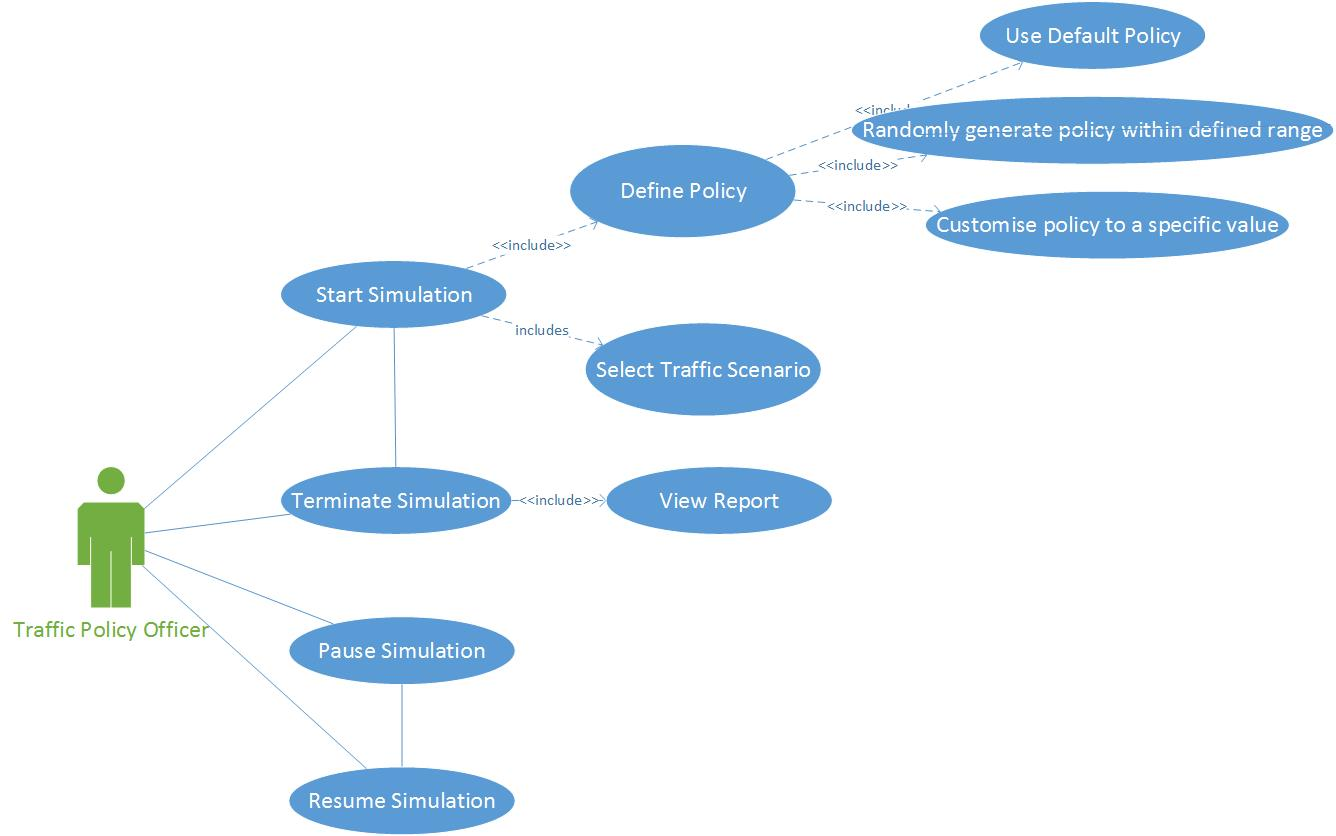
\includegraphics[width=16cm]{usecase} \caption{Use Case} \label{uc}
        \end{figure}
        \item Detailed Requirements 
        \begin{itemize}
            \item Controlled Map & Road network: User can choose multiple map options to simulate
                 \begin{itemize}[noitemsep]
	                    \item Junction: Simulate within a crossroad with 2 multi-lane and multi-direction roads. There is traffic light control at the crossroad.
	                    \item Town: Simulate within a larger town area which is a more complicated road network, including multiple roads, junctions, traffic lights. 
                    	\item Scalability: the program should allow adding more map options easily as required. 
	
    	\end{itemize}

        \item Vehicles: Simulate multiple types of vehicles, which include at least cars and ambulances (emergency vehicle) and at least three classes of driver’s behaviours (reckless, cautious, normal).

        \item Policy: the application must support at least fixed control policy (traffic light timing, speed limit). It should be scalable to variable control policy. The application provides users options to define the policy to be simulated:
            \begin{itemize}
                \item Default: default policy, which has speed limit 60mph and traffic light timing of 10s for Green Light/Red Light/Amber Light
                \item Random: User can simulate the policy which is randomly regenated within the user-defined range
                \item Customised: User can manually enter value for the policy.
    \end{itemize}

\item Simulation engine: must test the policies with different types of vehicles and drivers' behaviours in different levels of traffic density.
\item Report: Must provide the statistics and calculates metrics  for each simulation session as above.
\end{itemize}

        
    \end{itemize}
     Develop a simulation engine for testing traffic management
	policies
	\begin{itemize}[noitemsep]
	\item Should simulate individual vehicles (cars, coaches, buses etc.)
	operating in different parts of a road network (e.g. roundabouts,
	multi-lane junctions).
	\item Consider where vehicles enter road network and where they
	leave it.
	\item Consider individual behaviours (e.g. reckless, cautious, normal).
	\item Consider timing of journeys (based on purpose and patterns of
	use).
	\item Consider support for emergency services (e.g. prioritise
	ambulances at traffic lights).
	\item Allow different traffic management policies to be plugged in and
	compared.
	\item Decide on a time granularity for the simulation (e.g. 10 seconds).
	\item Each tick of the simulation clock will require all parts of the
	simulation to update.
	\item The simulation engine will record vehicle positions, new entries
	and exits and any other data and then update the state before
	moving to the next tick.
	\end{itemize}
	
    
    {\bf{Non-Functional Requirements:}} \newline
    
	
\subsection{Design}
In this section we will discuss the design process for this project. On the first week after the group was formed, we 

    \subsubsection{Planning}
    We set out the following feature for this application:
    
    \begin{itemize}[noitemsep]
    	\item FT-1: Map-Lane
    	\item FT-2: Map-Junction
    	\item FT-3: Map-Traffic Light
    	\item FT-4: Map-Road
    	\item FT-5: Map-Roundabout
    	\item FT-6: Map-Network Manager
    	\item FT-7: Map-Complex
    		\begin{itemize}
        	\item FT-7-1: Multiple roundabouts
        	\item FT-7-2: Multiple roundabouts, junctions, roads and lanes
        	\end{itemize}
    	\item FT-8: Vehicle-Generic Vehicle
    	\item FT-9: Vehicle-Cars
    	\item FT-10: Vehicle-Buses
    	\item FT-11: Vehicle-Traffic Light
    	\item FT-12: Vehicle-Accelerate/Decelerate
    	\item FT-13: Vehicle-Change Lane/Direction
    	\item FT-14: Vehicle-Driver's Behaviour
    	\item FT-15: Vehicle-Emergency
    	\item FT-16: Policy-Fixed Speed Limit and Fixed Traffic Light Time
    	\item FT-17: Policy-Variable Control Policy
    	\item FT-18: GUI-Lane
    	\item FT-19: GUI-Junction and traffic light
    	\item FT-20: GUI-Roundabout
    	\item FT-21: GUI-Multiple vehicles
    	\item FT-22: GUI-Animation
    	\item FT-23: Simulation Engine
    	    \begin{itemize}
        	\item FT-23-1: Simulation Engine Essential(?)
        	\item FT-23-2: Simulation Engine Optimal(?)
        	\end{itemize}
    	\item FT-24: Data Log and Analysis
   \end{itemize}

\noindent We divide the feature priority to Must Have and Could Have, 
\\
\textbf{Must Have:} FT-1, FT-2, FT-3, FT-4, FT-6, FT-8, FT-9, FT-11, FT-12, FT-13, FT-14, FT-15, FT-16, FT-18, FT-19, FT-21, FT-22, FT-23, FT-24
\\
\textbf{Could Have:} FT-5, FT-10, FT-17, FT-20
\\ \\
The milestone for each iteration and the functional requirement that we want to deliver can be seen in Table \ref{table:iteration} below. The class diagram from planning phase can be seen in Appendices figure \ref{fig:Planning}.

\begin{center}
% \begin{table}[!htb]

		
% 		\centering % used for cantering table
% 		\begin{tabular}{|p{1.8cm}|p{5cm}|p{1.2cm}|p{5cm}|} % centered columns
% 		\hline\hline %inserts double horizontal lines
% 		Milestone & Deliverable & Date & Dependant Upon \\ [0.5ex] % heading
% 		\hline
		
% 		1st Report & Intermediate Report complete (Iteration 0) & Feb 9 & Intermediate Planning and Initial Progress\\[1ex]
		
% 		Initial & Application Ready (Iteration 1) & Feb 18 & First iteration of bugs fixed. Iteration 1 features implemented. Program ready for unit test.  \\ [1ex]
		
% 		Mid & Application Ready (Iteration 2) & Mar 3 &  Second iteration of bugs fixed. Iteration 2 features implemented. Program ready for unit test.\\ [1ex]
		
% 		Pre-Final & Application ready (Iteration 3) & Mar 17 & All features and bugs fixed. Program finalised. \\[1ex]
		
% 		Final & Report complete and application ready (Iteration 4)  & Mar 31 & Completion of packaging and program. Final report ready. All testing done. \\[1ex] % [1ex] adds vertical space
% 		\hline
% 		\end{tabular}
% 		\caption{Planning: Project Milestones} % title of Table
% 		\label{table:milestones} % used to refer this table in the text
% 	\end{table}

\begin{table}[!htb]
		
		\centering
		%\begin{tabular}{p{2.5cm}|p{4cm}|p{2.5cm}|p{2.5cm}|p{2cm}}
		\begin{tabular}{|m{3cm}|m{2cm}|m{2cm}|m{2cm}|m{3cm}|}
		\hline
		\multicolumn{5}{ |>{\columncolor[gray]{0.8}}c|}{\textbf{Iterations}} \\
		\hline
		\textbf{Iteration 0} & \textbf{Iteration 1} & \textbf{Iteration 2} & \textbf{Iteration 3}& \textbf{Iteration 4} \\ \hline
		
		Requirements & FT-1 & FT-5 & FT-7-2 & Final Report\\ \hline
		
		System Architecture Design & FT-2 & FT-7-1 & FT-10 & Final Bug Fixing\\ \hline
		
		Component Detailed Design & FT-3 & FT-14 & FT-17 & Final Testing\\ \hline
		
		Initial Report & FT-4 & FT-15 & FT-22 & \\ \hline
		
		& FT-6 & FT-20 & FT-23-2 & \\ \hline
		
		& FT-18 & FT-21 && \\ \hline
		
		& FT-19 & FT-24 & &\\ \hline
		& FT-21 &&&\\ \hline
		& FT-8 &&& \\ \hline
		& FT-9 &&& \\ \hline
		& FT-11 &&& \\ \hline
		& FT-12 &&& \\ \hline
		& FT-13 &&& \\ \hline
		& FT-23-1 &&& \\ \hline
		& FT-16 &&&\\ \hline
		\end{tabular}
		\caption{Project Iteration (Planning phase)}
		\label{table:iteration} 
		\end{table}
\end{center}
 
 %insert class diagram
	
\section{Implementation} 
% st significant implementation details, focusing on those where unusual or detailed solutions were required. Quote code fragments where necessary, but remember that the full source code will be included as an appendix. Explain how you tested your software (e.g. unit testing) and the extent to which you tested it. If relevant to your project, explain performance issues and how you tackled them.
% This section of the report shall discusses the actual implementation of the traffic simulator system. The section will begin by discussing the initial prototypes that were developed and follow up with the technical discussion of the final implemented system.

This section of the report discusses about some of the implementation details that are deemed important to the project. The section is divided into different subsections.
\subsection{Overall Architecture}
This project was developed in Java. We decided to use Model-View-Controller(MVC) as the architectural pattern, and Singleton as the creational pattern. It is common to think of an application as having three main
layers such as presentation or user interface, application logic, and resource management. In MVC, the presentation
layer is split into controller and view. The most important separation is between presentation and
application logic. MVC encompasses more of the architecture of an application than is typical for a design pattern. Hence the term architectural pattern may be useful, or perhaps an aggregate design pattern.
    \begin{itemize}
    \item Model: The domain-specific representation of the information on which the application operates.
    The model is another name for the application logic layer (sometimes also called the
    domain layer). Application (or domain) logic adds meaning to raw data (e.g., calculating if today
    is the user’s birthday, or the totals, taxes and shipping charges for shopping cart items).
    Many applications use a persistent storage mechanism (such as a database) to store data.
    MVC does not specifically mention the resource management layer because it is understood
    to be underneath or encapsulated by the Model.
    \item View: Renders the model into a form suitable for interaction, typically a user interface
    element.
    \item Controller : Processes and responds to events, typically user actions, and may invoke changes
    on the model and view.
    \end{itemize}

The control flow in MVC generally works with the user interacts with the user interface in some way, a controller handles the input event from the user interface, and the controller accesses the model. In our application, (?)
Simulation Engine as the Controller, Vehicle, Policy and Road Network as the Model and the GUI as the View (?). 


\subsection{Development}
\subsubsection{GUI}

\subsubsection{Road Network}
What is road network
    \paragraph{Road}
    \textbf{Road Factory}\\
    \paragraph{Lane}
    \begin{itemize}[noitemsep]
    \item \textbf{LeftLane:} this  
    \item \textbf{RightLane:} this
    \item \textbf{SingleLane:} this
    \item \textbf{MiddleLane:} this  
    \item \textbf{LaneFactory:} this
    \end{itemize}
    \paragraph{Junction}
    \begin{itemize}[noitemsep]
    \item \textbf{PrePlannedRouteJuntion:} this  
    \item \textbf{TrafficLight:} this
    \item \textbf{TrafficLightWrapper:} this
    \end{itemize}
    
\subsubsection{Vehicle}
What is vehicle
\textbf{Vehicle Factory}\\


\subsubsection{Policy}        
\begin{itemize}[noitemsep]
\item \textbf{Policy} 
\item \textbf{SpeedLimit} 
\item \textbf{TrafficLightPolicy}
\end{itemize}

\subsubsection{Session Manager}
The Session Manager is the software component in charge of the session steps notifications. 
It was designed to be a monolithic component who launches notifications to any other when an arbitrary time period has passed, we will refer to this time as step. In order to accomplish the most appropriate design patterns to use are the Singleton and the Observer pattern.
The Session Manager component is divided into two parts. One is the Session.java and the SessionManager.java. 
The first file has the class who represents the actual object who keeps track of when a step has passed. It contains the thread safe mechanisms to increase and decrease the step size, so an external component may modify the size when convenient, allowing to speed up or slow down the beating of steps. It also contains a condition who allows an external component to pause the beating. The Session class inherits from the Java API class Observer. This means it has the pattern within ready to be used, therefore anyone could subscribe and start listening the Session notifications (the steps). For all the previous reasons, a Session object is meant to be run in its own thread, therefore it implements the Runnable interface.
The second file is the actual Session Manager. It works as the only entry point to any component who wants to know about the session steps. In order to ensure this, it follows the Singleton pattern. The Session Manager is the only object who knows about the Session, this means it is the only one able to create an instance of a Session thread. The Session Manager exposes the Session API in a thread safe manner when needed. Whenever a components ask the Session Manager to start a Session, it launches a new Session thread if there is none already running. When a session is stopped, the Session Manager


\subsubsection{Simulator Engine}
        
\begin{itemize}[noitemsep]
\item \textbf{Context} 
\item \textbf{SimulationEngine} is the engine that control the entire system and simulation.
\item \textbf{Context} is the list for all needed information.
\item \textbf{SimulationData} is the class for collecting all the data during the simulation iteration. Data including the number of vehicles, the number of vehicle that succeeded to arrived at the their destination, average speed from all the vehicles, the number of crashed between vehicle, and the traffic estimation. The detail calculation method for the traffic estimation will be discuss in \ref{rte}.
\end{itemize}.

\subsubsection{Road Traffic Estimation} \label{rte}
The methodology to calculate the road traffic estimation we derived from annual series of road traffic estimation that published by the Department for Transport. We simplified and did several adjustment to our simulation data to get the estimation number. Department of Transport uses manual traffic counts. this data then combined with information from a network of automatic traffic counter (ATCs) to calculate a series of annual average daily flows (AADF) for each count point. These daily flows then combined with road lengths to calculate the number of vehicle miles travelled each year by vehicle types, road category and region. In the document AADF major and minor road are separated as traffic volume is calculated differently for major and minor roads, however, for our calculation we use the simulation data. For every tick represent as 25,000,000 nanosecond, so we need 144 minutes to simulate 24 hours traffic. 
to convert the AADFs into traffic volume we multiply AADF with the link length, we then multiply it by the number of days in the year (365) to get an annual total. Link length is the total length of the network road link in km. For each lane section that we have, we decided that it will represent 3 meter in real life. Therefore, the link length calculate that from the number of lane section in the map and we multiply it by 0.003 km. 
\end{itemize}.
	
\subsection{Development Adjustment}
Several functions that we planned in our iteration before that changed
\begin{enumerate}[noitemsep]
	\item No Vehicle Bus 
	\item No Vehicle Emergency
	\item No Roundabout  
\end{enumerate}

\section{Team Work}
%Describe how you worked together, including the tools and processes you used to facilitate group work.
On the first sprint, or iteration 1, we managed to do almost all the tasks that we listed before. Since it's still initiation state, we mostly created different classes and objects that we thought we will need later. Files from policy (Policy, Speedlimit, Trafficlight), GUI (UIComponent, drawUI), road network (AbstractLaneSection, LaneFactory, LaneSection, LeftLane, MiddleLane, RightLane, SingleLane, ListOfListRoadImpl, Road, RoadFactory), main (SessionManager, SimulatorEngine, TrafficSimulatorApplication), and vehicle (Behaviour, Bus, Car, Direction, Emergency, Point, Vehicle, VehicleFactory, VehicleType). We also created JUnit test files for unit testing such as testpolicy, testlanesection, sessionmanagersprtest, sessionmanagertest and testvehicle. 

In the end of iteration 1 we decided to change our designed by moving all the control from the engine to the vehicle. Therefore the vehicle itself would have the method to accelerate and decelerate, and the behaviour towards traffic light. The decision making will still be on simulation engine but the behaviour will be declared on the vehicle itself. 
For the iteration 2, we added new classes. Files from: policy (TrafficLightColour), and roadnetwork (Junction, PrePlannedRouteJunction, TrafficLight). We also developed the GUI class again from scratch, because in iteration 1 we still unsure about the detail design and how the data flow will work from the simulation engine to the UI component. We deleted UIComponent and drawUI, and added GUIComponent, InitScreen, integertextfield, irenderer, simulationrender, simulationsetting). However, some of the tasks that we designated for this iteration could not be done and moved to the next sprint/iteration.  

We used Trello for the project management. Tasks in each iterations breaks down and assigned it to member. In the end of each iteration we have a meeting to discuss what are the tasks that we need to do for the next iteration. We created a list for each iteration, and wrote cards to put the task in. After the task is done, we can move it to the DONE list, so we know which task that have not finished yet. The unfinished task then moved to the next iteration, and added as the new workload.

In initial planning, we intend to have biweekly meeting, on Monday and Thursday. However, during development phase, we had a meeting almost three or four times a week, and increased to meet five to six times a week starting in iteration 3. We used the whatsapp group to arranged the meeting time and place. 

We used sharelatex to edit our final report together. This collaboration application work better than what we did for our initial report. We divided our part for the initial report into two groups, project description and project organisation. We then worked it separately and combined it in Github. This method appeared to created a lot of problem. We had a lot of document conflicts, from five people doing the edit the same file. Sharelatex is a good solution for this problem, since the group can collaborate in parallel and stimultaniously. 

\subsection{Work Load Division:}
Since the project will be relatively of small to medium size, in our initial planning, we decided that the group will facilitate job rotation at every iteration of development. This will be done to increase depth and breadth of understanding of the project by all members, as well as allow for a more flexible work distribution. In our first iteration we divided the tasks to 5 important components, such as Session Manager, Vehicle, Policy, Road, and GUI.

This strategy works perfectly fine until the end of iteration 2, but in the beginning of iteration 3, we change strategy to stop rotating the roles, and stick to the area because the deadline was approaching. The problem about this strategy is that we spend a lot of time to discuss specific logic together, rather than use the time to develop the code. We also need time to explaining the logic that the previous programmer to the next programmer. 

	
\section{Evaluation} %Critically evaluate your project: what worked well, and what didn’t? how did you do relative to your plan? what changes were the result of improved thinking and what changes were forced upon you? how did your team work together? etc. Note that you need to show that you understand the weaknesses in your work as well as its strengths. You may wish to identify relevant future work that could be done on your project.
\begin{enumerate}
	\item \textbf{Road development:} 
	\\@TODO
	\item \textbf{Simulation Engine development:} 
	\\@TODO
	\item \textbf{GUI:} 
	\\@TODO
\end{enumerate}

\subsection{Testing} 
%Explain how you tested your software (e.g. unit testing) and the extent to which you tested it. If relevant to your project, explain performance issues and how you tackled them.
@TODO
\\Test unit with JUnit. Test app with Black Box. 
Table~\ref{table:TestingTable} illustrates the bugs that were found within the system during black box testing tested by a random user and the team:
\begin{center}
	\begin{table}[!htb]
	\begin{tabular}{|m{7cm}|m{7cm}|}
		 \hline
		\multicolumn{2}{ |>{\columncolor[gray]{0.8}}c|}{\textbf{Black Box Testing}} \\ 
		\hline 
		 \centering \textbf{Bug} & \textbf{Status}\\\hline
		 &  \\  \hline
		
	\end{tabular}
	\caption{Testing Table}
		\label{table:TestingTable}
	\end{table}
\end{center}

\pagebreak
\subsection{Lessons Learned and Challenges}

The team feels that participating in the project was a very productive experience. It allowed team members to gain a first hand understanding of the techniques, concepts, and practices that are common in professional Software Development. It also allowed team members to put into practice the engineering and computing skills they have been learning about, to complete a meaningful project. 

However there were several aspects which the team feels lessons could be learned from.
These can be broken down into two categories, Engineering lessons and Teamwork lessons.

\paragraph{Engineering}

Engineering lessons involve things the team learned from the design, architecture, implementation, and testing of the code.

\begin{enumerate}
	
	\item \textbf{Overreach:}
	
	One of the most common lessons learned on computing projects is trying to do too much within a constrained period of time. It is understandable that, given a green field project, imaginative developers would be tempted to create expansive and open ended pieces of software. Unfortunately these projects tend to be bogged down with unnecessary components and a general sense of trying to do too much. This is a pitfall that the team is partially guilty of falling into. 
	
	At the beginning of the project, there was an optimistic feeling that the team could build a piece of traffic software comparable to commercially or academically available software. After a while of working on the project, it was decided that some of the \textit{would like to have} aspects should be dropped in favour of a more workable approach.
	
	The iterative Scrum style methodology \cite{website:Scrum-Alliance} the team adopted for development worked well in allowing us to respond to our changing goal. As after our first iteration we were able to see our overreach and realign our development goals. As our iterations progressed we were able to better understand our own abilities and limitations yet still create working piece of usable software at the end of each iteration.
	
	The main learning point of overreach is to set realistic constraints, but to allow for change. So that as your team creates software they are able to take advantage of new developments and progress not only the project but also their own abilities.
	
	\item \textbf{Vagueness of specification:}
	
	Similar to the problem of overreach is that of Vague Specification. Because the project had an open specification, it was the team's responsibility to whittle it down to a specific system. Initially the team was too vague about what they wanted their traffic simulator to be, too vague about the functional and non-functional requirements, too vague about what the team wanted to achieve with their product.
	
	The team believes that their Agile approach \cite{website:Agile-Manifesto} to development helped alleviate this issue. Because of the initial uncertainty over the purpose of the simulator, Agile helped them to refine their goals by emphasizing responsiveness over planning. Through successive iterations, the team was able to \textit{test the water} and get a feel for what purpose the project should achieve. To avoid \textit{scope creep} it was necessary for the team to be disciplined in remembering the agile principle of working software, and not introduce excess scope if \textit{'you ain't gonna need it'}.
	
	This wasn't a case of hacking a project together \textit{ad-hoc}. But a case of the team recognizing being in the situation of attempting a project with uncertain or undefined specification, and researching an established methodology for tackling these kinds of project. Then being pragmatic about adapting the methods to suit our needs.
	
	\item \textbf{Principles of Software Engineering}
	
	One of the things that helped the group overcome uncertainty in the project was to be faithful to a number of Software Engineering Principles that have become established within the Object Orientated software community. Following practices such as SOLID \cite{website:Principles-of-OOD} would allow the team to create a reusable, flexible, and robust code base, meaning that as the iterations went on the project would not need to be re-written with each slight change in desired outcome.
	
	Many of the early abstractions decided on by the team were clean and reusable. Such as the abstraction that a \textit{'Road'} is just an environment that a \textit{'Vehicle'} can be on, or that a traffic management \textit{'Policy'} is a rule or set of rules to be plugged into a simulation. These early abstractions allowed the team to be adaptive, in the beginning the team wanted an agent based Vehicle, however as the project developed they switched to a MVC based Vehicle. Because the Vehicle had a sound abstraction as simply an entity in an environment that moves from place to place, it was easily to substitute the \textit{'smart'} agent to a \textit{'dumb'} controlled object based vehicle, whilst allowing for future developers to extend the Vehicle abstraction into a more intelligent agent.
	
	Unfortunately, there were times in which the team was unable to avoid falling into bad habits and poor practices. A number of \textit{code smells} became apparent, for example the hard coding of algorithms for Junction behaviour which require large cyclomatic complexity. An excess of duplicated code. As well as the problem of \textit{contrived complexity}, by forcing design patterns into the code where perhaps there could be a simplified design. Some of the \textit{code smells} are recoverable through refactoring, code review, and extra documentation. The team is aware that these were practices they did not follow as well as they should.
	
	Another Agile principle followed by the team was that of Test Driven Development (TDD) \cite{website:Intro-TDD}. The team extensively used functional testing to verify the implementation of their work. By following a cycle of 
	
	Write Tests - Run Tests - \textbf {\textit{FAIL}} - Write code - Run Tests - \textbf {\textit{PASS}}. 
	
	The team was able to continually verify that their implemented algorithm logic, and object design decisions were as intended by the coders.
	
	The team was able to use it's extensive test suites in regression testing, by making sure that historical tests still passed after integrating components from more recent iterations.
	
	It could be noted that TDD was not utilized as extensively as could have been. However, many Agile practitioners would suggest that these methodologies are simply guidelines to be followed to the extent that they contribute to the project, and that you shouldn't attempt to \textit{force} them into projects that they don't fit into. The team felt that this was the most suitable approach to take. To use testing to fulfil the needs of the project rather than to force testing into areas that the team didn't think suited it. Despite not following TDD explicitly for some areas of the simulator, the team still used testing to verify and check those areas for example Visual testing was used for verification of the visual elements.
	
	The team did not make full use of functional testing frameworks which could have assisted with difficult to test components. Using a Mock Object framework such as Mockito could have assisted with creating tests to verify visual elements that were difficult to test using just JUnit.
	
	The team also didn't fully utilize the static analysis domain of testing. Using whitebox testing as well as blackbox testing could have allowed the team to find bugs unfindable through blackbox testing alone.
	
	The main lesson learned in terms of TDD was not to use as many different types of testing as are available, but to use testing to the extent to which it supports development of the program.
	
	
\end{enumerate}

\paragraph{Teamwork}

Teamwork lessons are those learned from the trial and error of working with others to complete a project that would be too big for each of us as individuals.

\begin{enumerate}
	
	\item \textbf{Communication}
	
	Importance of communication
	
	Team communicated very well from the start, overcame constraints like time difference of classes and location by using tech and having a good sense of proirity.
	
	\item \textbf{Division of Work}
	
	
	
	
\end{enumerate}

\subsubsection{Group Work Lessons Learned}
%What we learnt about group work and working together
@TODO

\pagebreak
\subsection{Future Work} 
%How the project could be extended
One of the most challenging aspects of any project is imagining what could be done, if the project was taken up by another team of engineers after the original team moves on to pastures new.
\\~\\
The team has discovered several paths that could be followed. Each of which would advance the base project into more specialized areas.
They can be broken down into two categories. Engineering improvements and Data gathering/simulation improvements.

\paragraph{Engineering}
Engineering improvements involve changes to the system Software that could better utilize engineering principals and practices.

\paragraph{Data}
Data based improvements involve giving the user greater control or access to the data generated by the simulation.\\

\begin{enumerate}
	
	\item \textbf{Parallelism:}
	\\
	
	Parallelism has emerged as an important concept in engineering, and more specifically in traffic simulation. Liu \cite{website:phy-ntnu-traffic-simulation} makes parallelism the key purpose of their project. Taking advantage of machines with multiple cores could allow for faster and more detailed simulations to be run. Perhaps by allowing vehicles or other objects within the simulation to be built as individual threads which would allow vehicles to act independently and concurrently within a map. Also by separating out the concerns of data gathering and simulation, if different threads were responsible for either aspect they could be more specialised.
	
	However it also requires more attention to detail when designing and writing code. As you must take care to synchronise shared data items to avoid pitfalls like deadlock and race conditions. This increased burden was one of the reasons the team decided against parallelization in their original project.
	
	The project's use of Java as it's primary programming language would allow future developers a convenient way into introducing parallelism. Java includes native, as well as third party, support for parallelism, such as the Fork/Join framework\cite{LeaForkJoin} as well as the new Java 8 Streams functionality\cite{website:Oracle-Java-8}, as well as native control libraries for concurrency controls.
	
	The modular approach the team took to designing the system architecture also facilitates the introduction of parallelism, because different modules could be parallelised independently.
	\\While the Test Driven Development approach would allow iterative introduction of parallelisation with the capacity to test if the new developments fit in with the accepted functionality tested in the original test suites.\\
	
	\item \textbf{External Libraries:}
	\\
	
	Another future improvement would be to include libraries and code from outside sources. The team decided early on that because one constraint of the project was for it to be \textit{the teams own work}, and because no credit would be received from using other's work, that the team would use as few external tools as possible, thus to avoid conflict. 
	
	Most notably, visualisation and data gathering and analysis tools could be used. Visualisation tools could improve the user experience by allowing a more immersive interaction with the simulation. Because of the team's Model-View-Controller approach to the architecture, and because the team followed software principles of separation of responsibilities, it would be easy for future developers to introduce other visualisation modules to the project.
	
	The visualisation provided by the TransModeler Project project \cite{website:caliper.com-transmodeler} is a good example of how improving visualisation is key to an enjoyable, productive, and useful piece of Traffic Simulation software.
	\\ Data gathering could be improved by using something like Log4j \cite{website:Apache-Log4j} to log and collect data from simulations. Data analysis could be improved by utilizing external libraries such as Apache Spark.
	
	The teams decision to use Java is key to the extensibility of the project. Java has a rich history of third party libraries being designed and built with 'free' software licenses, so that others can use them in their own work and avoid reinventing the wheel.
	
	The team's architectural design, which focuses on reusabilty, substitutability, and scalability would give future developers the opportunity to come in and introduce a wide variety of tools with very little code re-writing.\\
	
	\item \textbf{Distributed Road Network:}
	\\
	
	One of the original \textit{would like to have} aims of the project was to counter some of the scalability problems of other Traffic Simulation software \cite{SewWilMer10} by providing for a distributed road network. By allowing the simulation to scale to multiple machines would mean larger and more detailed simulations could be run. But at the same time keeping the ability for simulations to be run on a single machine, so that smaller simulations would not need to worry about consistency and distribution issues.
	
	Although the team decided that it would be detrimental to provided such functionality within the original project, due to time constraints and a limited number of iterations, and that it would be more productive to focus on the more fundamental aspects of Traffic Simulation software so that our imagined customers would have access to usable software as early as possible.
	
	However, because the team recognized the importance of overcoming the scalability problem they made it a goal to allow for future developers to introduce distributed deployment with as little complication as possible.
	
	The fundamental road network data structure kept the transitions between different roads and junctions as simple and lightweight as possible allowing those same transitions to be carried out over a network by introducing a transfer protocol to mimic the transition.\\
	
	\item \textbf{Agent Programming for Vehicle behaviour:}
	\\
	
	One of the key decisions made by the team was to focus on creating a Model-View-Controller architecture for the system. This, however, limited the scope for introducing independent \textit{agent based} behaviour for the vehicles being modelled.
	
	It was recognised that allowing for the introduction of independent agent behaviour could be crucial to future iterations of the project, if taken on by other development teams. As Traffic Simulation of greater complexity would require software agents to model the independent nature of vehicle users on a real road.
	
	For this reason, the team decided on an abstract design for \textit{vehicles}. Creating this abstraction would allow our implementation of vehicles to be swapped out for a more complex agent based implementation.\\
	
	\item \textbf{Machine Learning for Vehicle Behaviour and Data Analysis:}
	\\
	
	A further improvement to Vehicle behaviour could be found by utilizing machine learning.
	
	Again, because of the flexible approach the team took, it would be convenient for a future development team to take over and add machine learning to the vehicle behaviour. Also because of the well documented nature of the source code and the \textit{Clean Code} \cite{MartinRC08} approach the team took, a new team could understand the current state of the project and make improvements without first having to slog through and decipher the current state.
	
	As well as Vehicle behaviour, the Analytical side of the Traffic Simulator could be improved with machine learning tools.
	
	@TODO - Perhaps add some more stuff here?\\
	
	\item \textbf{User defined Maps:} 
	\\
	
	Due to iteration constraints, it was decided that the working product at the end of the final development cycle should only contain maps predefined by the team. This allowed the team to present a demonstration of a useful and working product.
	
	The team did however realise that the Traffic Simulators potential would be greatly diminished if users could not add and create their own maps. On further iterations, it would be possible and productive to create a feature for generating a users own map.
	
	Because of the evident usefulness of this feature, the team made efforts to allow integration to be a simple as possible. The intuitive way that maps are created as a data structure, and the convenient way that maps are translated and drawn by the visualisation component, mean that future development teams have an easier time of implementing user maps.\\
	
	
	\item \textbf{Integration with Third party APIs for Maps:} 
	\\
	
	Following on from user generated maps, a component that allows the Traffic Simulator to be integrated with pre existing map software could be very useful. If a user could select a section of Google Maps and have the features of that map parsed into a data structure usable by the Simulator. Users would have the ability to create and run simulations on existing road networks with greater simplicity than if they had to construct maps themselves.
	
	Combining a component for users to create and edit their own maps with a feature for extracting maps from pre existing map software would allow users to re engineer road networks, to simulate potential improvements to real life road systems.
	
\end{enumerate}

	
\subsection{Peer Assessment}
@TODO
	%In a simple table, allocate the 100 ‘points’ you are given to each team member. Valid values range from 0 to 100 inclusive. You may assign decimal values, but the entire points must add up to precisely 100. As stated at the beginning of the project, when awarding points to each member it would based on contribution, ...below is the grade table for each member totalling up to 100. 
\\As stated in the initial report peer assessment would be based on how much each team member was able to contribute based on their individual skills.	
\begin{center}
	\begin{tabular}[!htb]{|m{4cm}||m{0.9cm}|}
		\hline
		\multicolumn{2}{|>{\columncolor[gray]{0.8}}c|}{ \textbf{Peer Assessment}} \\  \hline
		 & 20\\  \hline
		 & 20 \\  \hline
		 & 20 \\  \hline
		 & 20 \\  \hline
		& 20\\  \hline
		& 100\\  \hline
	\end{tabular}
\end{center}	
\newpage


\bibliography{main}
\bibliographystyle{plain}


\newpage

\section{Appendices} % ALL THE EXTRA STUFF.

\subsection{Project Risk Table}
@TODO
\subsection{Class Diagrams}
@TODO
\subsection{Package Diagram}
@TODO
\subsection{Live Application}
@TODO
\subsection{Gantt Chart}
@TODO
\end{document} %END OF REPORT
=======
\documentclass[11pt]{article}
\usepackage[a4paper,pdftex]{geometry}
\usepackage[english]{babel}
\usepackage{xcolor,enumitem} 
\usepackage{graphicx}
\usepackage{tabu}
\usepackage{longtable}
\usepackage{array} % for m[{x cm} in tables
\usepackage[lofdepth,lotdepth]{subfig}
\usepackage{colortbl}

%--- for subsubsubsection
\usepackage{titlesec}
\setcounter{secnumdepth}{4}
\titleformat{\paragraph}
{\normalfont\normalsize\bfseries}{\theparagraph}{1em}{}
\titlespacing*{\paragraph}
{0pt}{3.25ex plus 1ex minus .2ex}{1.5ex plus .2ex}
%---

\begin{document}
	\begin{titlepage}
	\center
	\newcommand{\HRule}{\rule{\linewidth}{0.5mm}} 

        {\huge \bfseries Final Report}\\[0.4cm]
        	\ Team Keep It Clean
        
        {\large \today}\\[10cm] 
        
        \begin{minipage}{0.4\textwidth}
        		\emph{Authors:}\\
        			1474524/1	Retno Larasati\\
                    1581767/1	Ian Galna Johnson\\	
                    1579212/1	Thi Thanh Huong Ngo\\
                    1557762/1	Daniel Arturo Mendoza Hernandez\\
                    1530247/1	Abdelrahman Hamdy Hassan\\
        \end{minipage}

\end{titlepage}
\tableofcontents
\newpage
	
\section{Introduction}

[Todo: opening paragraph]

The report have seven sections. The first section is an introduction to the project, including the background, description, objectives, scope and methodology. In the second section we will talk about the literature and application that we reviewed in the preparation of the project. The third section will explains the requirements and designs of this project. The fourth section will explains the detail implementations, from overall architecture to the each (?) of the development, including the development adjustment that we made through out the project. The fifth section will explain about the team work and the work load division. In the sixth section we will discuss about the project evaluation, such as the system test, lesson learn, and possible future works. All additional documents thats relevant will be in section seven, for instance class diagrams,package diagram and Gantt chart. 

\subsection{Background}
Traffic simulation software plays an important role in defining the effective traffic management policies. A traffic policy must be simulated and verified before it is actually implemented in real life. Otherwise, it might harm road users’ safety and traffic efficiency. There are a lot of factors contributing to road accidents and traffic efficiency. The major factors include speed, traffic light timing and driver’s behaviours. For instance, in 2013, in the UK, 3,064 people were killed or seriously injured in crashes where speed was a factor.
Therefore, this project will simulate traffic management policies focusing on those 3 main factors ie. Speed limit; Traffic light timing; Driver's behaviours. The software will test different policies relating to these factors and analyse the traffic efficiency and safety in relation to traffic density, enforcement policy and driver's behaviours.

The analysis will be based on the average speed: average speed of vehicles in a session. This metric is to measure traffic efficiency and reliability.

In this report, we will explain how our traffic simulator works and how the simulator implements (what we implement? what our purposes)
	
\subsection{Descriptions}
%description of the project
This system will try to simulate the traffic with.

\subsection{Objectives}
Our initial objectives for this project where as follows:
\begin{itemize}[noitemsep]
\item Develop traffic simulator program with functional road system with vehicles, roads, junctions, intersections and traffic lights.
\item Analyse how the simulator working in emergency situation by creating emergency vehicle in the simulation session. (?)
\end{itemize}

\subsection{Scope}
The software is to simulate the traffic management policy following UK highway code which is left-lane oriented and using the speed limit within the range of speed limit defined in the UK highway code.
Within the constraints of time and resources, the project's scope includes:
\begin{itemize}[noitemsep]
\item Controlled Map: Minimum multiple-lane roads and a junction. It should support the scalability to a complex traffic network (ie. Multiple roundabouts, multiple junctions, multiple traffic lights, bus lane).
\item Vehicles: Simulate multiple types of vehicles, which include at least cars and ambulances (emergency vehicle) and at least three classes of driver’s behaviours (reckless, cautious, normal).
\item Policy: the project must support at least fixed control policy (traffic light timing, speed limit). It should be scalable to variable control policy.
\item Simulation engine: must test the policies with different levels of traffic density.
\item Report: Must provide the statistics and calculates metrics as above.
\end{itemize}

	
\subsection{Methodology}
\begin{enumerate}
\item Analysing: 
\item Planing and Organising:
    \begin{itemize}[noitemsep]
	\item Class Diagram
	\item Schedule: Gantt Chart
	\item Tasks management: Trello
	\end{itemize}
\item Developing:
	\begin{itemize}[noitemsep]
	\item Software: Java
	\item Source code: GitHub
	\end{itemize}
\item 	Evaluating:
	\begin{itemize}[noitemsep]
	\item Program
	\item Peer Assessment
	\end{itemize}
\item  	Reporting:
	\begin{itemize}[noitemsep]
	\item Documentation: LaTeX
	\item Presentation
	\end{itemize}
\end{enumerate}

\section{Review}

One of the traffic simulator reviewed was by Namekawa et al \cite{NameUeda05}. Even though there was a lot of road traffic simulation developed before, almost all them were developed with specific areas so they cannot be reused for simulation in the other area. Namekawa et al tried to create a general simulation system to analyse road traffic congestion of arbitrary areas. The general traffic simulation also wished to be not too complicated, with shorter simulation process time. They modeled the road network with such variable width portions that divided into three kinds of sub-roads as two side lines and a center line and also used a model of a cell automaton as one technique to realize microscopic model road traffic simulation in a city. [PARAPHRASING NEED]. [need to add more?]

From this system, the group got an insight to how to build the road network for a traffic simulation.  We also created different types of lanes to accommodate the traffic lane change. MiddleLane as the center line, LeftLane and RightLane as the side line. 

The other paper that reviewed was by Sewall et al \cite{SewWilMer10}. They modeled detailed 3D animations and visualization of traffic flows, fast method for efficient simulations of large-scale, real-world networks of traffic using continuum dynamics that maintains discrete vehicle information to display each vehicle.
Sewall approached this by adapting a single-lane continuum flow model to handle multi-lane traffic by introducing a novel model of lane changes and using a discrete visual representation for each vehicle and then compared the result with agent-based methods. [I don't know what we got from here?]


\newpage
\section{Requirements and Design}
\subsection{Requirement}
The following initial requirements come from the \textcolor{black}{\emph{Introductory Lecture Slides:}}\\
	{\bf{Technology:}}
	\begin{itemize}[noitemsep]
		\item Use whatever language / tools you see fit with 2 exceptions.
		\item All development of source code and documentation must be
		done through a public GitHub repository. Failure to do so will
		lead to a deduction of 25 marks from the final team grade.
		\item All documentation must be created with LATEX and handed in
		PDF format. Failure to do so will lead to a deduction of 25
		marks from the final team grade.
		\item Use the standard article class with the default margins and
		11pt font and produce the PDF with pdflatex.
	\end{itemize}
	
	{\bf{System Requirements:}} \newline
	\indent Develop a simulation engine for testing traffic management
	policies
	\begin{itemize}[noitemsep]
	\item Should simulate individual vehicles (cars, coaches, buses etc.)
	operating in different parts of a road network (e.g. roundabouts,
	multi-lane junctions).
	\item Consider where vehicles enter road network and where they
	leave it.
	\item Consider individual behaviours (e.g. reckless, cautious, normal).
	\item Consider timing of journeys (based on purpose and patterns of
	use).
	\item Consider support for emergency services (e.g. prioritise
	ambulances at traffic lights).
	\item Allow different traffic management policies to be plugged in and
	compared.
	\item Decide on a time granularity for the simulation (e.g. 10 seconds).
	\item Each tick of the simulation clock will require all parts of the
	simulation to update.
	\item The simulation engine will record vehicle positions, new entries
	and exits and any other data and then update the state before
	moving to the next tick.
	\end{itemize}
	
\subsection{Design}
In this section we will discuss the design process for this project. On the first week after the group was formed, we 

    \subsubsection{Planning}
    We set out the following feature for this application:
    
    \begin{itemize}[noitemsep]
    	\item FT-1: Map-Lane
    	\item FT-2: Map-Junction
    	\item FT-3: Map-Traffic Light
    	\item FT-4: Map-Road
    	\item FT-5: Map-Roundabout
    	\item FT-6: Map-Network Manager
    	\item FT-7: Map-Complex
    		\begin{itemize}
        	\item FT-7-1: Multiple roundabouts
        	\item FT-7-2: Multiple roundabouts, junctions, roads and lanes
        	\end{itemize}
    	\item FT-8: Vehicle-Generic Vehicle
    	\item FT-9: Vehicle-Cars
    	\item FT-10: Vehicle-Buses
    	\item FT-11: Vehicle-Traffic Light
    	\item FT-12: Vehicle-Accelerate/Decelerate
    	\item FT-13: Vehicle-Change Lane/Direction
    	\item FT-14: Vehicle-Driver's Behaviour
    	\item FT-15: Vehicle-Emergency
    	\item FT-16: Policy-Fixed Speed Limit and Fixed Traffic Light Time
    	\item FT-17: Policy-Variable Control Policy
    	\item FT-18: GUI-Lane
    	\item FT-19: GUI-Junction and traffic light
    	\item FT-20: GUI-Roundabout
    	\item FT-21: GUI-Multiple vehicles
    	\item FT-22: GUI-Animation
    	\item FT-23: Simulation Engine
    	    \begin{itemize}
        	\item FT-23-1: Simulation Engine Essential(?)
        	\item FT-23-2: Simulation Engine Optimal(?)
        	\end{itemize}
    	\item FT-24: Data Log and Analysis
   \end{itemize}

We divide the feature priority to Must Have and Could Have, 
\\ \\
\textbf{Must Have:} FT-1, FT-2, FT-3, FT-4, FT-6, FT-8, FT-9, FT-11, FT-12, FT-13, FT-14, FT-15, FT-16, FT-18, FT-19, FT-21, FT-22, FT-23, FT-24
\\ \\
\textbf{Could Have:} FT-5, FT-10, FT-17, FT-20
\\ \\
The milestone for each iteration and the functional requirement that we want to deliver can be seen in Table \ref{table:iteration} below. The class diagram from planning phase can be seen in Appendices figure \ref{fig:Planning}.

\begin{center}
% \begin{table}[!htb]

		
% 		\centering % used for cantering table
% 		\begin{tabular}{|p{1.8cm}|p{5cm}|p{1.2cm}|p{5cm}|} % centered columns
% 		\hline\hline %inserts double horizontal lines
% 		Milestone & Deliverable & Date & Dependant Upon \\ [0.5ex] % heading
% 		\hline
		
% 		1st Report & Intermediate Report complete (Iteration 0) & Feb 9 & Intermediate Planning and Initial Progress\\[1ex]
		
% 		Initial & Application Ready (Iteration 1) & Feb 18 & First iteration of bugs fixed. Iteration 1 features implemented. Program ready for unit test.  \\ [1ex]
		
% 		Mid & Application Ready (Iteration 2) & Mar 3 &  Second iteration of bugs fixed. Iteration 2 features implemented. Program ready for unit test.\\ [1ex]
		
% 		Pre-Final & Application ready (Iteration 3) & Mar 17 & All features and bugs fixed. Program finalised. \\[1ex]
		
% 		Final & Report complete and application ready (Iteration 4)  & Mar 31 & Completion of packaging and program. Final report ready. All testing done. \\[1ex] % [1ex] adds vertical space
% 		\hline
% 		\end{tabular}
% 		\caption{Planning: Project Milestones} % title of Table
% 		\label{table:milestones} % used to refer this table in the text
% 	\end{table}

\begin{table}[!htb]
		
		\centering
		%\begin{tabular}{p{2.5cm}|p{4cm}|p{2.5cm}|p{2.5cm}|p{2cm}}
		\begin{tabular}{|m{3cm}|m{2cm}|m{2cm}|m{2cm}|m{3cm}|}
		\hline
		\multicolumn{5}{ |>{\columncolor[gray]{0.8}}c|}{\textbf{Iterations}} \\
		\hline
		\textbf{Iteration 0} & \textbf{Iteration 1} & \textbf{Iteration 2} & \textbf{Iteration 3}& \textbf{Iteration 4} \\ \hline
		
		Requirements & FT-1 & FT-5 & FT-7-2 & Final Report\\ \hline
		
		System Architecture Design & FT-2 & FT-7-1 & FT-10 & Final Bug Fixing\\ \hline
		
		Component Detailed Design & FT-3 & FT-14 & FT-17 & Final Testing\\ \hline
		
		Initial Report & FT-4 & FT-15 & FT-22 & \\ \hline
		
		& FT-6 & FT-20 & FT-23-2 & \\ \hline
		
		& FT-18 & FT-21 && \\ \hline
		
		& FT-19 & FT-24 & &\\ \hline
		& FT-21 &&&\\ \hline
		& FT-8 &&& \\ \hline
		& FT-9 &&& \\ \hline
		& FT-11 &&& \\ \hline
		& FT-12 &&& \\ \hline
		& FT-13 &&& \\ \hline
		& FT-23-1 &&& \\ \hline
		& FT-16 &&&\\ \hline
		\end{tabular}
		\caption{Project Iteration (Planning phase)}
		\label{table:iteration} 
		\end{table}
\end{center}
 
 %insert class diagram
	
\section{Implementation} 
% st significant implementation details, focusing on those where unusual or detailed solutions were required. Quote code fragments where necessary, but remember that the full source code will be included as an appendix. Explain how you tested your software (e.g. unit testing) and the extent to which you tested it. If relevant to your project, explain performance issues and how you tackled them.
% This section of the report shall discusses the actual implementation of the traffic simulator system. The section will begin by discussing the initial prototypes that were developed and follow up with the technical discussion of the final implemented system.

This section of the report discusses about some of the implementation details that are deemed important to the project. The section is divided into different subsections.
\subsection{Overall Architecture}
This project was developed in Java. We decided to use Model-View-Controller(MVC) as the architectural pattern, and Singleton as the creational pattern. It is common to think of an application as having three main
layers such as presentation or user interface, application logic, and resource management. In MVC, the presentation
layer is split into controller and view. The most important separation is between presentation and
application logic. MVC encompasses more of the architecture of an application than is typical for a design pattern. Hence the term architectural pattern may be useful, or perhaps an aggregate design pattern.
    \begin{itemize}
    \item Model: The domain-specific representation of the information on which the application operates.
    The model is another name for the application logic layer (sometimes also called the
    domain layer). Application (or domain) logic adds meaning to raw data (e.g., calculating if today
    is the user’s birthday, or the totals, taxes and shipping charges for shopping cart items).
    Many applications use a persistent storage mechanism (such as a database) to store data.
    MVC does not specifically mention the resource management layer because it is understood
    to be underneath or encapsulated by the Model.
    \item View: Renders the model into a form suitable for interaction, typically a user interface
    element.
    \item Controller : Processes and responds to events, typically user actions, and may invoke changes
    on the model and view.
    \end{itemize}

The control flow in MVC generally works with the user interacts with the user interface in some way, a controller handles the input event from the user interface, and the controller accesses the model. In our application, (?)
Simulation Engine as the Controller, Vehicle, Policy and Road Network as the Model and the GUI as the View (?). 


\subsection{Development}
\subsubsection{GUI}

\subsubsection{Road Network}
What is road network
    \paragraph{Road}
    \textbf{Road Factory}\\
    \paragraph{Lane}
    \begin{itemize}[noitemsep]
    \item \textbf{LeftLane:} this  
    \item \textbf{RightLane:} this
    \item \textbf{SingleLane:} this
    \item \textbf{MiddleLane:} this  
    \item \textbf{LaneFactory:} this
    \end{itemize}
    \paragraph{Junction}
    \begin{itemize}[noitemsep]
    \item \textbf{PrePlannedRouteJuntion:} this  
    \item \textbf{TrafficLight:} this
    \item \textbf{TrafficLightWrapper:} this
    \end{itemize}
    
\subsubsection{Vehicle}
Vehicle here is a component in which the simulation will analyse. We created enumerator files such as Behaviour for driver behaviour, Direction for the information of the direction that the vehicle take, and VehicleType to differentiate between Car, Bus, and Emergency Vehicle. We decided that the vehicle object would not be the one that makes decision of how and where to go. All logic goes to SimulationEngine.



\subsubsection{Policy}        
\begin{itemize}[noitemsep]
\item \textbf{Policy} 
\item \textbf{SpeedLimit} 
\item \textbf{TrafficLightPolicy}
\end{itemize}

\subsubsection{Session Manager}
The Session Manager is the software component in charge of the session steps notifications.


\subsubsection{Simulator Engine}
        
\begin{itemize}[noitemsep]
\item \textbf{Context} 
\item \textbf{SimulationEngine} is the engine that control the entire system and simulation.
\item \textbf{Context} is the list for all needed information.
\item \textbf{SimulationData} is the class for collecting all the data during the simulation iteration. Data including the number of vehicles, the number of vehicle that succeeded to arrived at the their destination, average speed from all the vehicles, the number of crashed between vehicle, and the traffic estimation. The detail calculation method for the traffic estimation will be discuss in \ref{rte}.
\end{itemize}.

\subsubsection{Road Traffic Estimation} \label{rte}
The methodology to calculate the road traffic estimation we derived from annual series of road traffic estimation that published by the Department for Transport. We simplified and did several adjustment to our simulation data to get the estimation number. Department of Transport uses manual traffic counts. this data then combined with information from a network of automatic traffic counter (ATCs) to calculate a series of annual average daily flows (AADF) for each count point. These daily flows then combined with road lengths to calculate the number of vehicle miles travelled each year by vehicle types, road category and region. In the document AADF major and minor road are separated as traffic volume is calculated differently for major and minor roads, however, for our calculation we use the simulation data. For every tick represent as 25,000,000 nanosecond, so we need 144 minutes to simulate 24 hours traffic. 
to convert the AADFs into traffic volume we multiply AADF with the link length, we then multiply it by the number of days in the year (365) to get an annual total. Link length is the total length of the network road link in km. For each lane section that we have, we decided that it will represent 3 meter in real life. Therefore, the link length calculate that from the number of lane section in the map and we multiply it by 0.003 km. 
\subsection{Development Adjustment}
Several functions that we planned in our iteration before that changed
\begin{enumerate}[noitemsep]
	\item No Vehicle Bus 
	\item No Vehicle Emergency
	\item No Roundabout  
\end{enumerate}

\section{Team Work}
%Describe how you worked together, including the tools and processes you used to facilitate group work.
On the first sprint, or iteration 1, we managed to do almost all the tasks that we listed before. Since it's still initiation state, we mostly created different classes and objects that we thought we will need later. Files from policy (Policy, Speedlimit, Trafficlight), GUI (UIComponent, drawUI), road network (AbstractLaneSection, LaneFactory, LaneSection, LeftLane, MiddleLane, RightLane, SingleLane, ListOfListRoadImpl, Road, RoadFactory), main (SessionManager, SimulatorEngine, TrafficSimulatorApplication), and vehicle (Behaviour, Bus, Car, Direction, Emergency, Point, Vehicle, VehicleFactory, VehicleType). We also created JUnit test files for unit testing such as testpolicy, testlanesection, sessionmanagersprtest, sessionmanagertest and testvehicle. 

In the end of iteration 1 we decided to change our designed by moving all the control from the engine to the vehicle. Therefore the vehicle itself would have the method to accelerate and decelerate, and the behaviour towards traffic light. The decision making will still be on simulation engine but the behaviour will be declared on the vehicle itself. 
For the iteration 2, we added new classes. Files from: policy (TrafficLightColour), and roadnetwork (Junction, PrePlannedRouteJunction, TrafficLight). We also developed the GUI class again from scratch, because in iteration 1 we still unsure about the detail design and how the data flow will work from the simulation engine to the UI component. We deleted UIComponent and drawUI, and added GUIComponent, InitScreen, integertextfield, irenderer, simulationrender, simulationsetting). However, some of the tasks that we designated for this iteration could not be done and moved to the next sprint/iteration.  

We used Trello for the project management. Tasks in each iterations breaks down and assigned it to member. In the end of each iteration we have a meeting to discuss what are the tasks that we need to do for the next iteration. We created a list for each iteration, and wrote cards to put the task in. After the task is done, we can move it to the DONE list, so we know which task that have not finished yet. The unfinished task then moved to the next iteration, and added as the new workload.

In initial planning, we intend to have biweekly meeting, on Monday and Thursday. However, during development phase, we had a meeting almost three or four times a week, and increased to meet five to six times a week starting in iteration 3. We used the whatsapp group to arranged the meeting time and place. 

We used sharelatex to edit our final report together. This collaboration application work better than what we did for our initial report. We divided our part for the initial report into two groups, project description and project organisation. We then worked it separately and combined it in Github. This method appeared to created a lot of problem. We had a lot of document conflicts, from five people doing the edit the same file. Sharelatex is a good solution for this problem, since the group can collaborate in parallel and stimultaniously. 

\subsection{Work Load Division:}
Since the project will be relatively of small to medium size, in our initial planning, we decided that the group will facilitate job rotation at every iteration of development. This will be done to increase depth and breadth of understanding of the project by all members, as well as allow for a more flexible work distribution. In our first iteration we divided the tasks to 5 important components, such as Session Manager, Vehicle, Policy, Road, and GUI.

This strategy works perfectly fine until the end of iteration 2, but in the beginning of iteration 3, we change strategy to stop rotating the roles, and stick to the area because the deadline was approaching. The problem about this strategy is that we spend a lot of time to discuss specific logic together, rather than use the time to develop the code. We also need time to explaining the logic that the previous programmer to the next programmer. 

	
\section{Evaluation} %Critically evaluate your project: what worked well, and what didn’t? how did you do relative to your plan? what changes were the result of improved thinking and what changes were forced upon you? how did your team work together? etc. Note that you need to show that you understand the weaknesses in your work as well as its strengths. You may wish to identify relevant future work that could be done on your project.
\begin{enumerate}
	\item \textbf{Road development:} 
	\\@TODO
	\item \textbf{Simulation Engine development:} 
	\\@TODO
	\item \textbf{GUI:} 
	\\@TODO
\end{enumerate}

\subsection{Testing} 
%Explain how you tested your software (e.g. unit testing) and the extent to which you tested it. If relevant to your project, explain performance issues and how you tackled them.
@TODO
\\Test unit with JUnit. Test app with Black Box. 
Table~\ref{table:TestingTable} illustrates the bugs that were found within the system during black box testing tested by a random user and the team:
\begin{center}
	\begin{table}[!htb]
	\begin{tabular}{|m{7cm}|m{7cm}|}
		 \hline
		\multicolumn{2}{ |>{\columncolor[gray]{0.8}}c|}{\textbf{Black Box Testing}} \\ 
		\hline 
		 \centering \textbf{Bug} & \textbf{Status}\\\hline
		 &  \\  \hline
		
	\end{tabular}
	\caption{Testing Table}
		\label{table:TestingTable}
	\end{table}
\end{center}

\subsection{Lessons Learned and Challenges} 
%How did you do relative to your plan?
@TODO


\subsubsection{Group Work Lessons Learned}
%What we learnt about group work and working together
@TODO

	
\subsection{Future Work} 
%How the project could be extended
One of the most challenging aspects of any project is imagining what could be done, if the project was taken up by another team of engineers after the original team moves on to pastures new.
\\~\\
The team has discovered several paths that could be followed. Each of which would advance the base project into more specialized areas.
They can be broken down into two categories. Engineering improvements and Data gathering/simulation improvements.

\paragraph{Engineering}
Engineering improvements involve changes to the system Software that could better utilize engineering principals and practices.
\begin{enumerate}
	\item \textbf{Parallelism:}
	\\~\\
	Parallelism has emerged as an important concept in engineering, and more specifically in traffic simulation. Liu \cite{website:phy-ntnu-traffic-simulation} makes parallelism the key purpose of their project. Taking advantage of machines with multiple cores could allow for faster and more detailed simulations to be run. Perhaps by allowing vehicles or other objects within the simulation to be built as individual threads which would allow vehicles to act independently and concurrently within a map. Also by separating out the concerns of data gathering and simulation, if different threads were responsible for either aspect they could be more specialised.
	
	However it also requires more attention to detail when designing and writing code. As you must take care to synchronise shared data items to avoid pitfalls like deadlock and race conditions. This increased burden was one of the reasons the team decided against parallelization in their original project.
	
	The project's use of Java as it's primary programming language would allow future developers a convenient way into introducing parallelism. Java includes native, as well as third party, support for parallelism, such as the Fork/Join framework\cite{LeaForkJoin} as well as the new Java 8 Streams functionality\cite{website:Oracle-Java-8}, as well as native control libraries for concurrency controls.
	
	The modular approach the team took to designing the system architecture also facilitates the introduction of parallelism, because different modules could be parallelised independently.
	\\While the Test Driven Development approach would allow iterative introduction of parallelisation with the capacity to test if the new developments fit in with the accepted functionality tested in the original test suites.
	
	\item \textbf{Use of External Libraries:}
	\\ Another future improvement would be to include libraries and code from outside sources. Most notably, visualisation and data gathering and analysis tools. Visualisation tools could improve the user experience by allowing a more immersive interaction with the simulation. The visualisation provided by the TransModeler Project project \cite{website:caliper.com-transmodeler} is a good example of how improving visualisation is key to an enjoyable, productive, and useful piece of Traffic Simulation software.
	\item \textbf{Distibuted Road Network:}
	\item \textbf{User defined maps:} 
	\\@TODO
	\\add user designed maps
	\item \textbf{Integration with Third party APIs:} 
	\\@TODO
	\\add draw maps from google maps API or something similar
\end{enumerate}

	
\subsection{Peer Assessment}
@TODO
	%In a simple table, allocate the 100 ‘points’ you are given to each team member. Valid values range from 0 to 100 inclusive. You may assign decimal values, but the entire points must add up to precisely 100. As stated at the beginning of the project, when awarding points to each member it would based on contribution, ...below is the grade table for each member totalling up to 100. 
\\As stated in the initial report peer assessment would be based on how much each team member was able to contribute based on their individual skills.	
\begin{center}
	\begin{tabular}[!htb]{|m{4cm}||m{0.9cm}|}
		\hline
		\multicolumn{2}{|>{\columncolor[gray]{0.8}}c|}{ \textbf{Peer Assessment}} \\  \hline
		 & 20\\  \hline
		 & 20 \\  \hline
		 & 20 \\  \hline
		 & 20 \\  \hline
		& 20\\  \hline
		& 100\\  \hline
	\end{tabular}
\end{center}	
\newpage


\bibliography{main}
@TODO
\bibliographystyle{plain}


\newpage

\section{Appendices} % ALL THE EXTRA STUFF.

\subsection{Project Risk Table}
@TODO
\subsection{Class Diagrams}
\begin{figure}[!htb]
\begin{tabular}{cc}
		\subfloat[User Diagram]{
		    \setlength{\fboxsep}{0pt}%
			\setlength{\fboxrule}{1pt}%
			\fbox{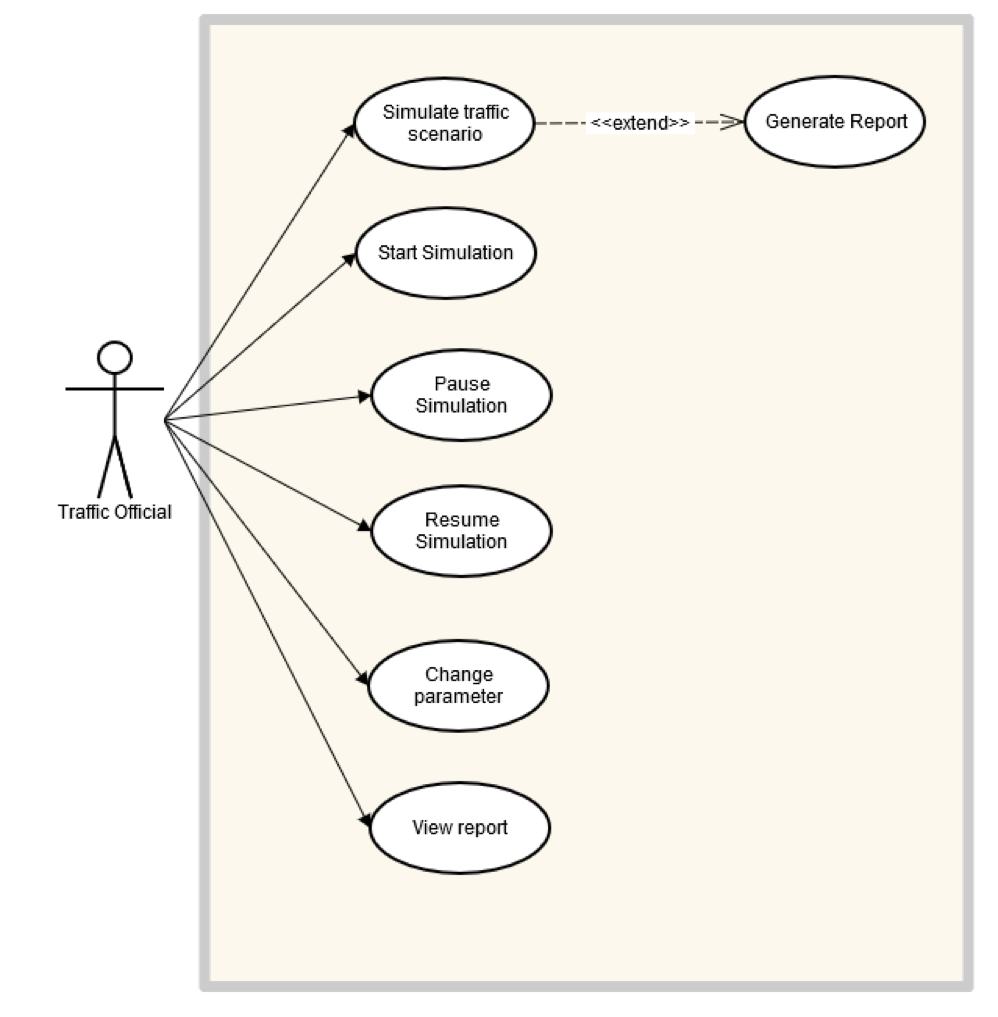
\includegraphics[width=0.45\linewidth]{Picture1}}
			\label{subfig:cd1}
		}&
		\subfloat[]{
		    \setlength{\fboxsep}{0pt}%
			\setlength{\fboxrule}{1pt}%
			\fbox{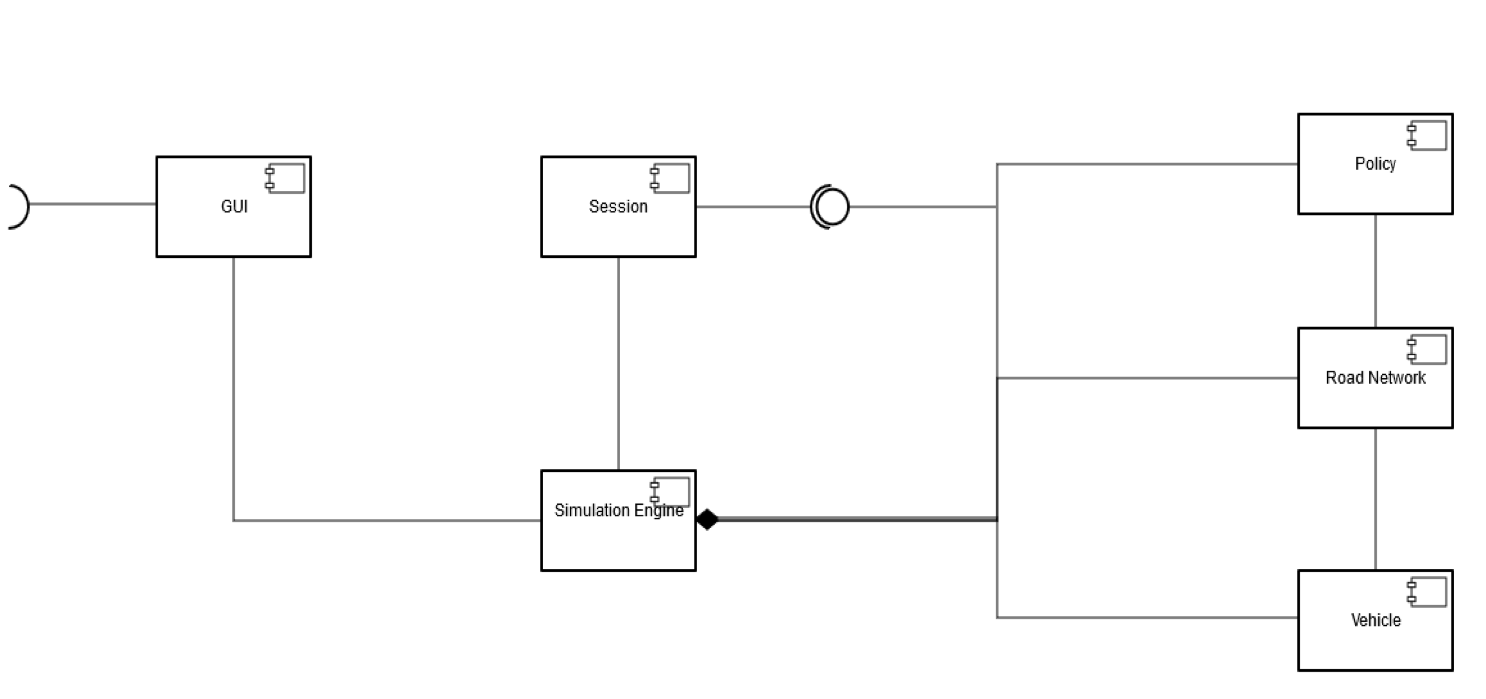
\includegraphics[width=0.45\linewidth]{Picture2}}
			\label{subfig:cd2}
		}\\
		\subfloat[]{
			\setlength{\fboxsep}{0pt}%
			\setlength{\fboxrule}{1pt}%
			\fbox{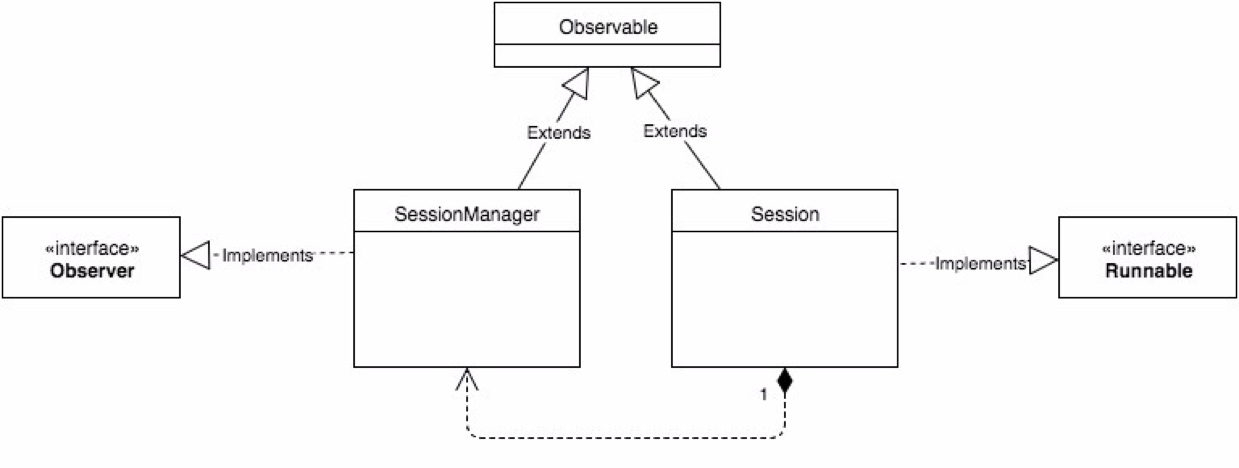
\includegraphics[width=0.45\linewidth]{Picture3}}
			\label{subfig:cd3}
		}&
		\subfloat[]{
			\setlength{\fboxsep}{0pt}%
			\setlength{\fboxrule}{1pt}%
			\fbox{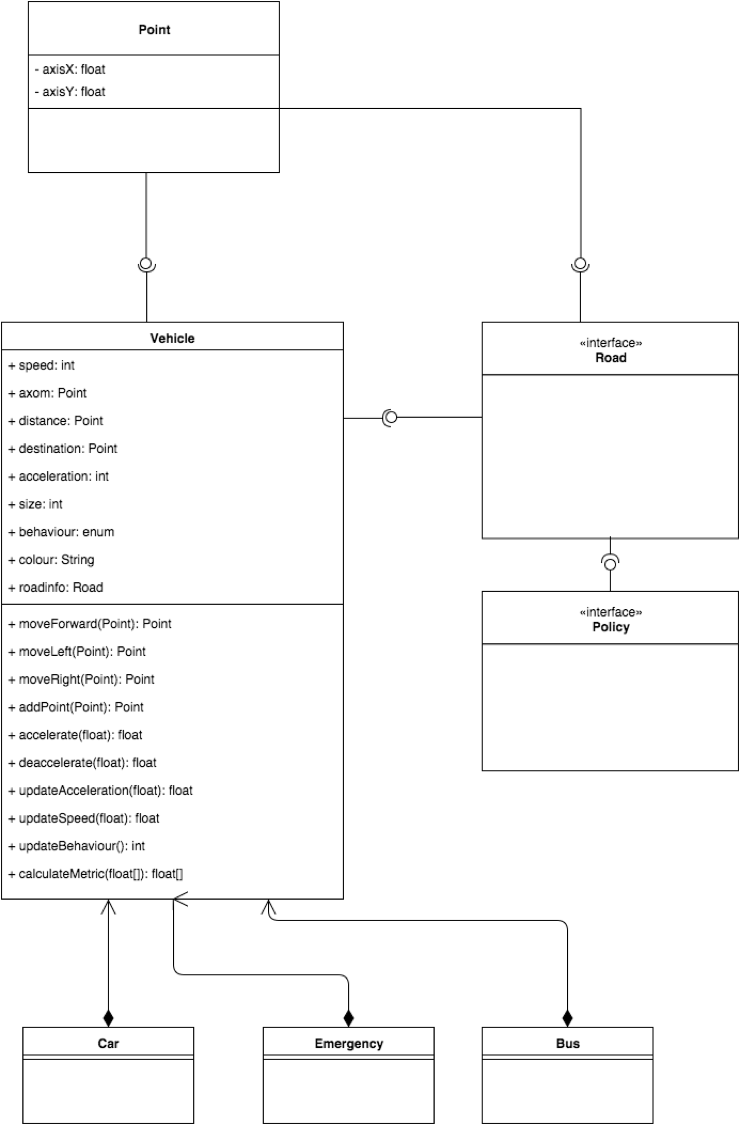
\includegraphics[width=8cm, height=6cm]{Picture4}}
			\label{subfig:cd4}
		}\\
		\subfloat[]{
			\setlength{\fboxsep}{0pt}%
			\setlength{\fboxrule}{1pt}%
			\fbox{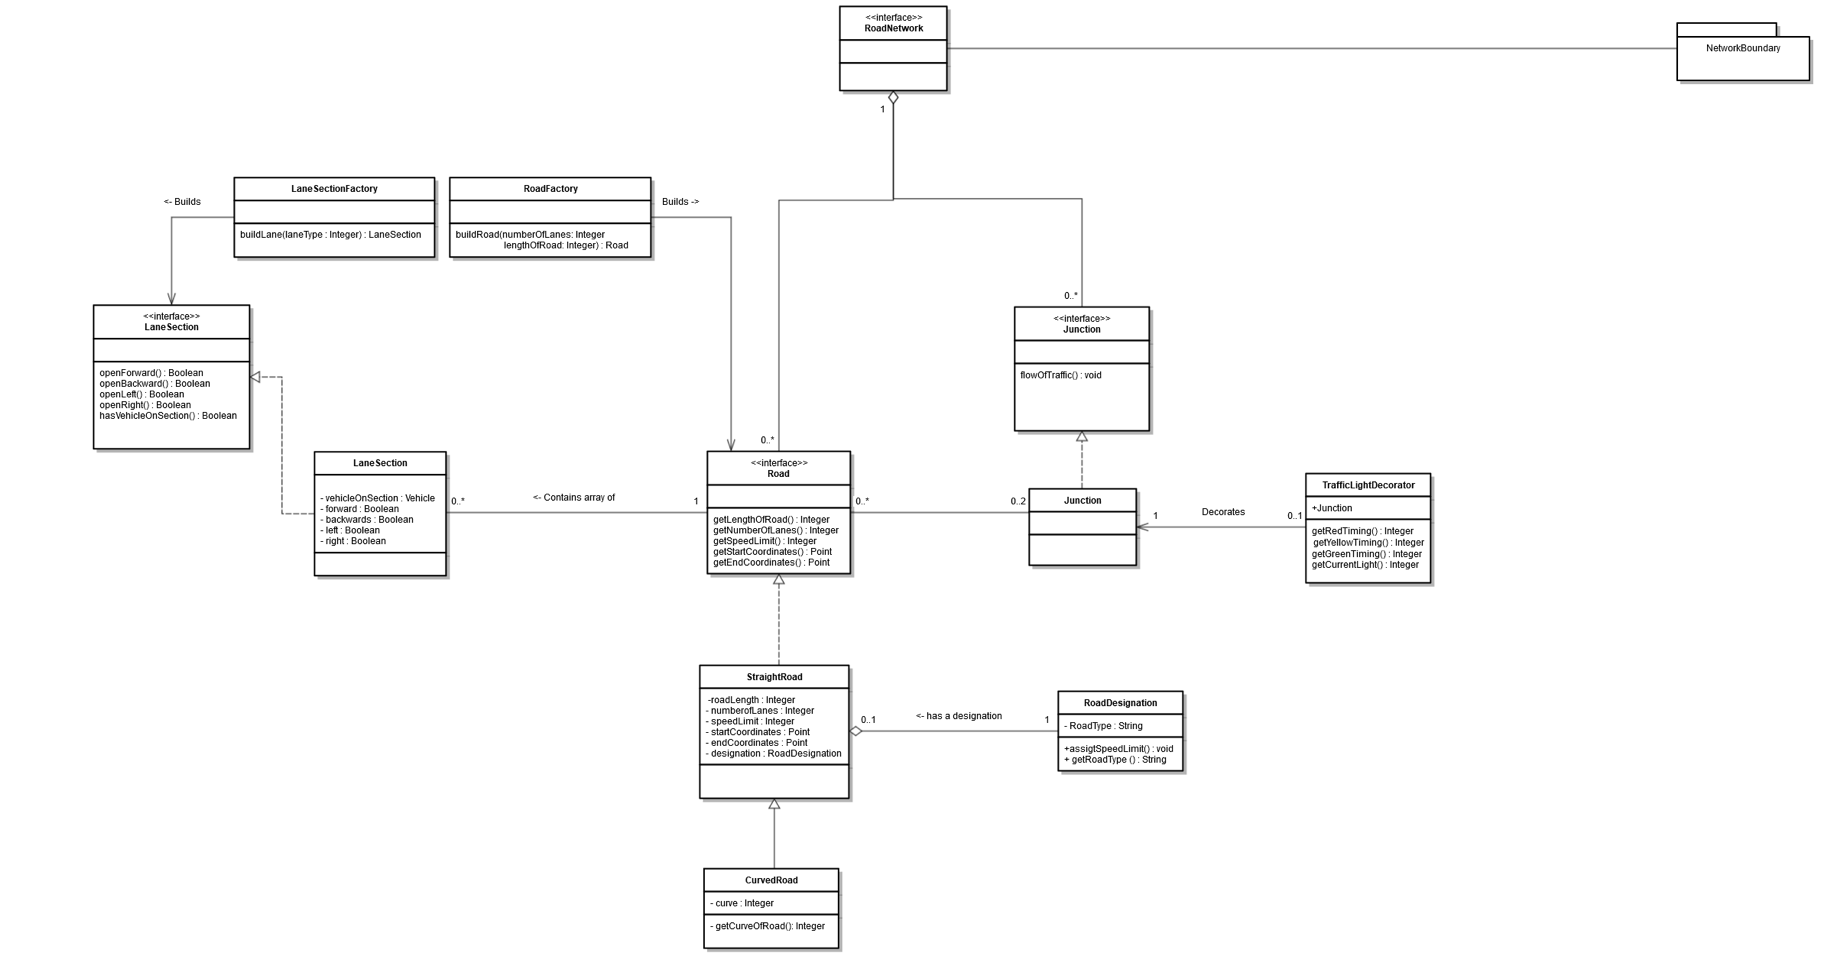
\includegraphics[width=0.45\linewidth]{Picture5}}
			\label{subfig:cd5}
		}
		\subfloat[]{
			\setlength{\fboxsep}{0pt}%
			\setlength{\fboxrule}{1pt}%
			\fbox{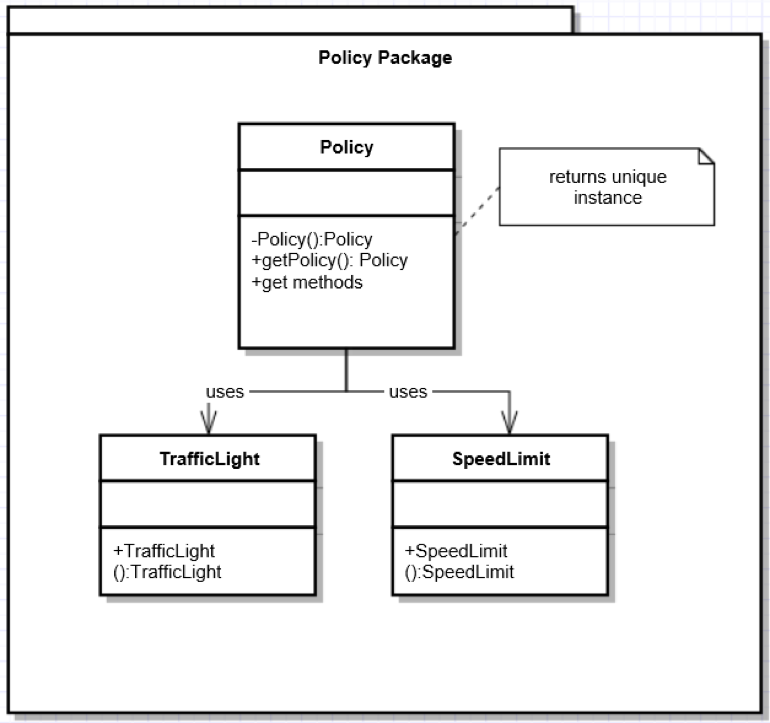
\includegraphics[width=0.45\linewidth]{Picture6}}
			\label{subfig:cd6}
		}
		\end{tabular}
		\caption[]{Planning Class Diagrams}
		\label{fig:Planning}
\end{figure}
\subsection{Package Diagram}
@TODO
\subsection{Live Application}
@TODO
\subsection{Gantt Chart}
@TODO


% \begin{center}
% \begin{longtabu} to \textwidth {|
%     X[4,l]|
%     X[3,c]|
%     X[8,l]|}
%     \hline
%     \textbf{Author} & \textbf{Date} & \textbf{Message} \ \hline
% retnolaras & 2016-01-24 & first commit \\ \hline
% Daniel Mendoza & 2016-01-25 & Update README.md \\ \hline
% retnolaras & 2016-01-28 & Initial Report \\ \hline
% Daniel Mendoza & 2016-01-29 & Merge remote-tracking branch `origin/daniel-arturo-mendoza-patch-1' \\ \hline
% Daniel Mendoza & 2016-01-29 & Session Manager \\ \hline
% Daniel Mendoza & 2016-01-29 & Merge remote-tracking branch `retnolaras/master' \\ \hline
% Daniel Mendoza & 2016-01-29 & Fixing Null pointers when starting and stopping the session. A new session object is now created every time a session starts. This session object is set to null when the session is stopped. Th garbage collector should handle it. \\ \hline
% retnolaras & 2016-01-30 & Merge pull request \#1 from daniel-arturo-mendoza/master \\ \hline
% igalna & 2016-02-01 & Initial Commit. \\ \hline
% igalna & 2016-02-01 & Package renaming for improved readability \\ \hline
% igalna & 2016-02-01 & kcl.keepitclean.test.roadnetwork \\ \hline
% igalna & 2016-02-01 & remove .class files from changes \\ \hline
% igalna & 2016-02-01 & .gitignore \\ \hline
% igalna & 2016-02-01 & TestRoadNetwork \\ \hline
% igalna & 2016-02-01 & gitignore \\ \hline
% igalna & 2016-02-01 & removed .class files form the bin directory \\ \hline
% igalna & 2016-02-01 & .gitignore \\ \hline
% igalna & 2016-02-01 & added bin folder to gitignore \\ \hline
% igalna & 2016-02-01 & Lane Section is the base object of a road network. \\ \hline
% retnolaras & 2016-02-02 & new initial report \\ \hline
% retnolaras & 2016-02-02 & section 1.3 and 1.4 \\ \hline
% Daniel Mendoza & 2016-02-02 & Merge remote-tracking branch `retnolaras/master' \\ \hline
% retnolaras & 2016-02-03 & Merge pull request \#2 from igalna/master \\ \hline
% retnolaras & 2016-02-03 & section 1.1 \\ \hline
% retnolaras & 2016-02-03 & coordinate and vehicle class \\ \hline
% retnolaras & 2016-02-03 & etc \\ \hline
% retnolaras & 2016-02-03 & Merge remote-tracking branch `origin/master' \\ \hline
% Daniel Mendoza & 2016-02-03 & adding info tom management, technical and test approaches. \\ \hline
% Daniel Mendoza & 2016-02-03 & Scrum \\ \hline
% Daniel Mendoza & 2016-02-03 & Merge remote-tracking branch `retnolaras/master' into daniel-arturo-mendoza-patch-1 \\ \hline
% retnolaras & 2016-02-03 & Merge pull request \#3 from daniel-arturo-mendoza/master \\ \hline
% Daniel Mendoza & 2016-02-03 & Roles \\ \hline
% Daniel Mendoza & 2016-02-03 & Merge branch `master' into daniel-arturo-mendoza-patch-1 \\ \hline
% Daniel Mendoza & 2016-02-03 & Technology and Quality \\ \hline
% Daniel Mendoza & 2016-02-03 & Merge remote-tracking branch `retnolaras/master' into daniel-arturo-mendoza-patch-1 \\ \hline
% retnolaras & 2016-02-04 & Merge pull request \#4 from daniel-arturo-mendoza/daniel-arturo-mendoza-patch-1 \\ \hline
% AbdoHassan1994 & 2016-02-04 & Create InitialReportGP.tex \\ \hline
% retnolaras & 2016-02-04 & delete some stuff from 1.1 and 1.2 \\ \hline
% Daniel Mendoza & 2016-02-04 & Merge remote-tracking branch `retnolaras/master' into daniel-arturo-mendoza-patch-1 \\ \hline
% Daniel Mendoza & 2016-02-04 & summarize \\ \hline
% retnolaras & 2016-02-04 & edit 1.1 \\ \hline
% retnolaras & 2016-02-04 & Merge pull request \#6 from daniel-arturo-mendoza/daniel-arturo-mendoza-patch-1 \\ \hline
% retnolaras & 2016-02-04 & Revert ``delete some stuff from 1.1 and 1.2'' \\ \hline
% retnolaras & 2016-02-04 & new \\ \hline
% retnolaras & 2016-02-04 & Merge remote-tracking branch `origin/master' \\ \hline
% AbdoHassan1994 & 2016-02-04 & Create InitialReportGP.tex \\ \hline
% retnolaras & 2016-02-04 & ignore pdf file \\ \hline
% AbdoHassan1994 & 2016-02-04 & Create InitialReportGP.tex \\ \hline
% retnolaras & 2016-02-04 & Merge pull request \#7 from AbdoHassan1994/patch-1 \\ \hline
% retnolaras & 2016-02-04 & remove table 1. \\ \hline
% retnolaras & 2016-02-04 & remove table 1 and edit 1.3 \\ \hline
% retnolaras & 2016-02-04 & merge stuff \\ \hline
% igalna & 2016-02-04 & Updated Initial report with section relating to handling the peer assessment \\ \hline
% igalna & 2016-02-04 & Initial report log files \\ \hline
% retnolaras & 2016-02-05 & Merge pull request \#8 from igalna/master \\ \hline
% retnolaras & 2016-02-05 & newest merge \\ \hline
% Daniel Mendoza & 2016-02-05 & Merge remote-tracking branch `retnolaras/master' into daniel-arturo-mendoza-patch-1 \\ \hline
% igalna & 2016-02-05 & Added the Conflict resolution section of the Initial Report Document \\ \hline
% igalna & 2016-02-05 & .log file for Initialreport \\ \hline
% retnolaras & 2016-02-06 & compacting the table \\ \hline
% retnolaras & 2016-02-06 & - \\ \hline
% retnolaras & 2016-02-06 & - \\ \hline
% retnolaras & 2016-02-06 & Delete InitialReportGP.pdf \\ \hline
% retnolaras & 2016-02-06 & Merge remote-tracking branch `origin/master' \\ \hline
% retnolaras & 2016-02-06 & Merge branch `pr/5' \\ \hline
% retnolaras & 2016-02-06 & Merge remote-tracking branch `origin/master' \\ \hline
% retnolaras & 2016-02-06 & add conflict handling \\ \hline
% retnolaras & 2016-02-08 & correcting typos \\ \hline
% igalna & 2016-02-08 & Merge remote-tracking branch `upstream/master' \\ \hline
% AbdoHassan1994 & 2016-02-08 & Merge remote-tracking branch `retnolaras/master' \\ \hline
% AbdoHassan1994 & 2016-02-08 & summary \\ \hline
% retnolaras & 2016-02-08 & Merge pull request \#10 from AbdoHassan1994/master \\ \hline
% Daniel Mendoza & 2016-02-08 & adding comments 1 \\ \hline
% Daniel Mendoza & 2016-02-08 & Merge remote-tracking branch `retnolaras/master' into daniel-arturo-mendoza-patch-1 \\ \hline
% igalna & 2016-02-08 & Merge remote-tracking branch `upstream/master' \\ \hline
% igalna & 2016-02-08 & updated local repo from master \\ \hline
% retnolaras & 2016-02-08 & edited initial progress \\ \hline
% rosiengo & 2016-02-08 & Merge remote-tracking branch `refs/remotes/retnolaras/master' \\ \hline
% retnolaras & 2016-02-08 & edited typo \\ \hline
% Daniel Mendoza & 2016-02-08 & Merge branch `retnolaras/master' into daniel-arturo-mendoza-patch-1 \\ \hline
% retnolaras & 2016-02-08 & changed some terms \\ \hline
% retnolaras & 2016-02-08 & Merge pull request \#11 from rosiengo/master \\ \hline
% rosiengo & 2016-02-09 & Merge remote-tracking branch `refs/remotes/retnolaras/master' \\ \hline
% rosiengo & 2016-02-09 & policy \\ \hline
% rosiengo & 2016-02-09 & policy test \\ \hline
% AbdoHassan1994 & 2016-02-09 & Merge pull request \#1 from retnolaras/master \\ \hline
% AbdoHassan1994 & 2016-02-09 & added sentences \\ \hline
% retnolaras & 2016-02-09 & Merge pull request \#13 from AbdoHassan1994/master \\ \hline
% rosiengo & 2016-02-10 & uml policy \\ \hline
% rosiengo & 2016-02-10 & updated policy code \\ \hline
% retnolaras & 2016-02-10 & Merge pull request \#12 from rosiengo/master \\ \hline
% igalna & 2016-02-10 & Merge remote-tracking branch `upstream/master' \\ \hline
% Daniel Mendoza & 2016-02-10 & Merge branch `retnolaras/master' into daniel-arturo-mendoza-patch-1 \\ \hline
% AbdoHassan1994 & 2016-02-15 & Merge remote-tracking branch `retnolaras/master' \\ \hline
% rosiengo & 2016-02-15 & new policy \\ \hline
% AbdoHassan1994 & 2016-02-15 & Create readme \\ \hline
% igalna & 2016-02-15 & Rename of TestRoadNetwork to TestLaneSection \\ \hline
% igalna & 2016-02-15 & TestLaneSection \\ \hline
% AbdoHassan1994 & 2016-02-15 & add files \\ \hline
% igalna & 2016-02-15 & AbstractLaneSection \\ \hline
% igalna & 2016-02-15 & Concrete implementations of the different LaneSections \\ \hline
% retnolaras & 2016-02-15 & Merge pull request \#14 from rosiengo/master \\ \hline
% retnolaras & 2016-02-15 & Merge pull request \#15 from AbdoHassan1994/patch-2 \\ \hline
% igalna & 2016-02-15 & LaneFactory class \\ \hline
% Daniel Mendoza & 2016-02-15 & Merge branch `retnolaras/master' into daniel-arturo-mendoza-patch-1 \\ \hline
% igalna & 2016-02-15 & Merge remote-tracking branch `upstream/master' \\ \hline
% retnolaras & 2016-02-15 & Merge pull request \#16 from igalna/master \\ \hline
% rosiengo & 2016-02-15 & NEW POLICY \\ \hline
% rosiengo & 2016-02-15 & ADD COMMENTS FOR USAGE GUIDELINES \\ \hline
% retnolaras & 2016-02-15 & Merge pull request \#17 from rosiengo/master \\ \hline
% Daniel Mendoza & 2016-02-16 & Merge branch `retnolaras/master' into daniel-arturo-mendoza-patch-1 \\ \hline
% igalna & 2016-02-16 & Amended Package structure \\ \hline
% retnolaras & 2016-02-18 & move some class \\ \hline
% Daniel Mendoza & 2016-02-18 & Merge branch `retnolaras/master' into daniel-arturo-mendoza-patch-1 \\ \hline
% igalna & 2016-02-19 & Test cases for Roads \\ \hline
% igalna & 2016-02-19 & Tests for Road \\ \hline
% igalna & 2016-02-19 & LaneSection \\ \hline
% igalna & 2016-02-19 & RoadFactory \\ \hline
% igalna & 2016-02-19 & Implementation of a Road \\ \hline
% igalna & 2016-02-19 & Vehicle implementation with a concrete instead of Abstract Vehicle \\ \hline
% igalna & 2016-02-19 & Merge remote-tracking branch `upstream/master' \\ \hline
% retnolaras & 2016-02-19 & Merge pull request \#18 from igalna/master \\ \hline
% Daniel Mendoza & 2016-02-20 & Merge branch `retnolaras/master' into daniel-arturo-mendoza-patch-1 \\ \hline
% Daniel Mendoza & 2016-02-21 & Synchronization and test cases. \\ \hline
% AbdoHassan1994 & 2016-02-21 & Merge pull request \#2 from AbdoHassan1994/files \\ \hline
% Daniel Mendoza & 2016-02-21 & Moving file into another package. \\ \hline
% retnolaras & 2016-02-21 & vehicle factory \\ \hline
% Daniel Mendoza & 2016-02-21 & Merge branch `retnolaras/master' into daniel-arturo-mendoza-patch-1 \\ \hline
% retnolaras & 2016-02-21 & Merge pull request \#19 from daniel-arturo-mendoza/daniel-arturo-mendoza-patch-1 \\ \hline
% Daniel Mendoza & 2016-02-21 & Merge branch `retnolaras/master' into daniel-arturo-mendoza-patch-1 \\ \hline
% retnolaras & 2016-02-21 & VehicleType \\ \hline
% Daniel Mendoza & 2016-02-21 & Merge branch `retnolaras/master' into daniel-arturo-mendoza-patch-1 \\ \hline
% retnolaras & 2016-02-21 & change Road to Lane \\ \hline
% Daniel Mendoza & 2016-02-21 & Indentation changes. Implementing Singleton Pattern. \\ \hline
% Daniel Mendoza & 2016-02-21 & Lane Factory \\ \hline
% Daniel Mendoza & 2016-02-21 & Simulator Engine \\ \hline
% Daniel Mendoza & 2016-02-21 & Merge branch `retnolaras/master' into daniel-arturo-mendoza-patch-1 \\ \hline
% rosiengo & 2016-02-22 & Merge pull request \#1 from retnolaras/master \\ \hline
% rosiengo & 2016-02-22 & update policy code and test \\ \hline
% retnolaras & 2016-02-22 & Merge pull request \#20 from daniel-arturo-mendoza/daniel-arturo-mendoza-patch-1 \\ \hline
% rosiengo & 2016-02-22 & test \\ \hline
% retnolaras & 2016-02-22 & Merge pull request \#23 from AbdoHassan1994/master \\ \hline
% AbdoHassan1994 & 2016-02-22 & Added initial Code for GUI component. \\ \hline
% retnolaras & 2016-02-22 & Merge pull request \#24 from AbdoHassan1994/master \\ \hline
% Daniel Mendoza & 2016-02-22 & Merge branch `retnolaras/master' into daniel-arturo-mendoza-patch-1 \\ \hline
% AbdoHassan1994 & 2016-02-22 & add files in right location \\ \hline
% retnolaras & 2016-02-22 & Merge pull request \#25 from AbdoHassan1994/master \\ \hline
% Daniel Mendoza & 2016-02-22 & Merge branch `retnolaras/master' into daniel-arturo-mendoza-patch-1 \\ \hline
% retnolaras & 2016-02-22 & master \\ \hline
% rosiengo & 2016-02-22 & Revert ``update policy code and test'' \\ \hline
% rosiengo & 2016-02-22 & Revert ``test'' \\ \hline
% rosiengo & 2016-02-22 & policy \\ \hline
% retnolaras & 2016-02-22 & Policy Test and changes on policy.java and speed limit.java \\ \hline
% retnolaras & 2016-02-22 & add VehicleTest \\ \hline
% rosiengo & 2016-02-23 & updated policy \\ \hline
% rosiengo & 2016-02-23 & Merge remote-tracking branch `refs/remotes/retnolaras/master' \\ \hline
% Daniel Mendoza & 2016-02-24 & Merge branch `retnolaras/master' into daniel-arturo-mendoza-patch-1 \\ \hline
% retnolaras & 2016-02-24 & Merge pull request \#28 from rosiengo/master \\ \hline
% AbdoHassan1994 & 2016-02-25 & update draw function \\ \hline
% AbdoHassan1994 & 2016-02-25 & Modified UI component \\ \hline
% rosiengo & 2016-02-25 & fixed error \\ \hline
% rosiengo & 2016-02-25 & Merge remote-tracking branch `refs/remotes/retnolaras/master' \\ \hline
% rosiengo & 2016-02-25 & bugs \\ \hline
% igalna & 2016-02-25 & Added a TestSuite class for all the Test classes from sprint 1. \\ \hline
% igalna & 2016-02-25 & Merge remote-tracking branch `upstream/master' \\ \hline
% retnolaras & 2016-02-25 & Merge pull request \#29 from rosiengo/master \\ \hline
% igalna & 2016-02-26 & Merge remote-tracking branch `upstream/master' \\ \hline
% rosiengo & 2016-02-26 & Merge remote-tracking branch `refs/remotes/retnolaras/master' \\ \hline
% retnolaras & 2016-02-28 & change name trafficLight to trafficLightPolicy \\ \hline
% retnolaras & 2016-02-28 & resolve conflict \\ \hline
% retnolaras & 2016-02-28 & add TrafficLightSection \\ \hline
% rosiengo & 2016-02-29 & Merge remote-tracking branch `refs/remotes/retnolaras/master' \\ \hline
% Daniel Mendoza & 2016-02-29 & Merge branch `retnolaras/master' into daniel-arturo-mendoza-patch-1 \\ \hline
% igalna & 2016-02-29 & Merge remote-tracking branch `upstream/master' \\ \hline
% retnolaras & 2016-03-01 & encapsulate axom \\ \hline
% igalna & 2016-03-01 & Merge remote-tracking branch `upstream/master' \\ \hline
% igalna & 2016-03-01 & Commit of updated ListOfListsRoadImpl \\ \hline
% retnolaras & 2016-03-01 & Merge pull request \#30 from AbdoHassan1994/master \\ \hline
% igalna & 2016-03-01 & Added Test class for the Junction \\ \hline
% retnolaras & 2016-03-01 & update vehicle \\ \hline
% igalna & 2016-03-01 & Added getVehicle method to AbstractLaneSection \\ \hline
% retnolaras & 2016-03-01 & public \\ \hline
% rosiengo & 2016-03-01 & GUI \\ \hline
% rosiengo & 2016-03-01 & Merge remote-tracking branch `refs/remotes/retnolaras/master' \\ \hline
% igalna & 2016-03-01 & Edited ListOfListsRoadImpl to change name of setStartCoordinate \\ \hline
% rosiengo & 2016-03-01 & gui \\ \hline
% rosiengo & 2016-03-01 & Revert ``GUI'' \\ \hline
% rosiengo & 2016-03-01 & Revert ``Revert''GUI``'' \\ \hline
% rosiengo & 2016-03-01 & Revert ``Revert''Revert ``GUI''``'' \\ \hline
% igalna & 2016-03-01 & Implementation of PrePlannedRouteJunction \\ \hline
% igalna & 2016-03-01 & Merge remote-tracking branch `upstream/master' \\ \hline
% rosiengo & 2016-03-01 & gui \\ \hline
% retnolaras & 2016-03-01 & Merge pull request \#31 from igalna/master \\ \hline
% retnolaras & 2016-03-01 & Merge pull request \#32 from rosiengo/master \\ \hline
% rosiengo & 2016-03-01 & Merge remote-tracking branch `refs/remotes/retnolaras/master' \\ \hline
% retnolaras & 2016-03-01 & TrafficLightJunction \\ \hline
% AbdoHassan1994 & 2016-03-03 & Update Car.java \\ \hline
% rosiengo & 2016-03-03 & Merge remote-tracking branch `refs/remotes/retnolaras/master' \\ \hline
% retnolaras & 2016-03-03 & Merge pull request \#33 from AbdoHassan1994/patch-3 \\ \hline
% AbdoHassan1994 & 2016-03-03 & CarPosition \\ \hline
% AbdoHassan1994 & 2016-03-03 & Update Position.java \\ \hline
% retnolaras & 2016-03-03 & Merge pull request \#34 from AbdoHassan1994/master \\ \hline
% AbdoHassan1994 & 2016-03-03 & Update position \\ \hline
% Daniel Mendoza & 2016-03-03 & Merge branch `retnolaras/master' into daniel-arturo-mendoza-patch-1 \\ \hline
% Daniel Mendoza & 2016-03-03 & Context and IContext commit \\ \hline
% rosiengo & 2016-03-03 & Merge remote-tracking branch `refs/remotes/retnolaras/master' \\ \hline
% retnolaras & 2016-03-03 & Merge pull request \#35 from AbdoHassan1994/master \\ \hline
% rosiengo & 2016-03-04 & Merge remote-tracking branch `refs/remotes/retnolaras/master' \\ \hline
% retnolaras & 2016-03-04 & Merge pull request \#36 from daniel-arturo-mendoza/daniel-arturo-mendoza-patch-1 \\ \hline
% Daniel Mendoza & 2016-03-04 & Merge branch `retnolaras/master' into daniel-arturo-mendoza-patch-1 \\ \hline
% retnolaras & 2016-03-04 & move traffic light to junction \\ \hline
% Daniel Mendoza & 2016-03-04 & Merge branch `retnolaras/master' into daniel-arturo-mendoza-patch-1 \\ \hline
% Daniel Mendoza & 2016-03-04 & fixing syntax errors \\ \hline
% Daniel Mendoza & 2016-03-04 & Fixing syntax errors \\ \hline
% AbdoHassan1994 & 2016-03-04 & add relative position ( interms of lane , roadsection and road ) to the car \\ \hline
% retnolaras & 2016-03-04 & Merge pull request \#37 from daniel-arturo-mendoza/daniel-arturo-mendoza-patch-1 \\ \hline
% retnolaras & 2016-03-04 & Merge pull request \#38 from AbdoHassan1994/patch-4 \\ \hline
% Daniel Mendoza & 2016-03-04 & Merge branch `retnolaras/master' into daniel-arturo-mendoza-patch-1 \\ \hline
% Daniel Mendoza & 2016-03-04 & move method \\ \hline
% retnolaras & 2016-03-04 & Merge pull request \#39 from daniel-arturo-mendoza/daniel-arturo-mendoza-patch-1 \\ \hline
% Daniel Mendoza & 2016-03-04 & Merge branch `retnolaras/master' into daniel-arturo-mendoza-patch-1 \\ \hline
% AbdoHassan1994 & 2016-03-04 & add functionality \\ \hline
% retnolaras & 2016-03-04 & Merge pull request \#41 from AbdoHassan1994/patch-5 \\ \hline
% Daniel Mendoza & 2016-03-05 & Merge branch `retnolaras/master' into daniel-arturo-mendoza-patch-1 \\ \hline
% rosiengo & 2016-03-05 & Merge remote-tracking branch `refs/remotes/retnolaras/master' \\ \hline
% AbdoHassan1994 & 2016-03-05 & Add LookAhead function \\ \hline
% retnolaras & 2016-03-05 & Merge pull request \#43 from AbdoHassan1994/patch-6 \\ \hline
% retnolaras & 2016-03-05 & edit errors + typos \\ \hline
% AbdoHassan1994 & 2016-03-05 & Change LookAhead Impl \\ \hline
% retnolaras & 2016-03-06 & Merge pull request \#44 from AbdoHassan1994/patch-7 \\ \hline
% AbdoHassan1994 & 2016-03-06 & Update SimulatorEngine.java \\ \hline
% retnolaras & 2016-03-06 & Merge pull request \#45 from AbdoHassan1994/patch-8 \\ \hline
% rosiengo & 2016-03-06 & Merge remote-tracking branch `refs/remotes/retnolaras/master' \\ \hline
% rosiengo & 2016-03-06 & gui \\ \hline
% rosiengo & 2016-03-06 & delete unused gui files \\ \hline
% rosiengo & 2016-03-06 & gui \\ \hline
% AbdoHassan1994 & 2016-03-06 & Update SimulatorEngine.java \\ \hline
% retnolaras & 2016-03-06 & Merge pull request \#46 from rosiengo/master \\ \hline
% retnolaras & 2016-03-06 & Merge pull request \#47 from AbdoHassan1994/patch-9 \\ \hline
% AbdoHassan1994 & 2016-03-06 & update \\ \hline
% AbdoHassan1994 & 2016-03-06 & update Driver program \\ \hline
% retnolaras & 2016-03-06 & Merge pull request \#48 from AbdoHassan1994/patch-10 \\ \hline
% retnolaras & 2016-03-06 & Merge pull request \#49 from AbdoHassan1994/patch-11 \\ \hline
% rosiengo & 2016-03-07 & Merge remote-tracking branch `refs/remotes/retnolaras/master' \\ \hline
% retnolaras & 2016-03-07 & Merge pull request \#51 from rosiengo/master \\ \hline
% rosiengo & 2016-03-07 & integration \\ \hline
% retnolaras & 2016-03-07 & Merge pull request \#52 from rosiengo/master \\ \hline
% AbdoHassan1994 & 2016-03-07 & Update SimulatorEngine.java \\ \hline
% retnolaras & 2016-03-07 & Merge pull request \#53 from AbdoHassan1994/patch-13 \\ \hline
% Daniel Mendoza & 2016-03-07 & Merge branch `retnolaras/master' into daniel-arturo-mendoza-patch-1 \\ \hline
% Daniel Mendoza & 2016-03-07 & Merge branch `retnolaras/master' into daniel-arturo-mendoza-patch-1 \\ \hline
% retnolaras & 2016-03-07 & update TrafficLight junction \\ \hline
% retnolaras & 2016-03-07 & edit policy \\ \hline
% Daniel Mendoza & 2016-03-07 & promoting Abdo's changes \\ \hline
% rosiengo & 2016-03-07 & gui + constants \\ \hline
% retnolaras & 2016-03-07 & Merge pull request \#54 from daniel-arturo-mendoza/daniel-arturo-mendoza-patch-1 \\ \hline
% retnolaras & 2016-03-07 & Merge pull request \#55 from rosiengo/master \\ \hline
% rosiengo & 2016-03-07 & Merge remote-tracking branch `refs/remotes/retnolaras/master' \\ \hline
% Daniel Mendoza & 2016-03-07 & adding getContext method to engine \\ \hline
% retnolaras & 2016-03-07 & Merge pull request \#56 from daniel-arturo-mendoza/daniel-arturo-mendoza-patch-1 \\ \hline
% retnolaras & 2016-03-07 & Merge pull request \#57 from rosiengo/master \\ \hline
% retnolaras & 2016-03-07 & get context \\ \hline
% Daniel Mendoza & 2016-03-07 & adding setRenderer \\ \hline
% retnolaras & 2016-03-07 & Merge pull request \#58 from daniel-arturo-mendoza/daniel-arturo-mendoza-patch-1 \\ \hline
% Daniel Mendoza & 2016-03-07 & InitScreen changes \\ \hline
% rosiengo & 2016-03-07 & Merge remote-tracking branch `refs/remotes/retnolaras/master' \\ \hline
% retnolaras & 2016-03-07 & Merge pull request \#59 from daniel-arturo-mendoza/daniel-arturo-mendoza-patch-1 \\ \hline
% Daniel Mendoza & 2016-03-07 & Merge branch `retnolaras/master' into daniel-arturo-mendoza-patch-1 \\ \hline
% rosiengo & 2016-03-07 & Merge remote-tracking branch `refs/remotes/retnolaras/master' \\ \hline
% rosiengo & 2016-03-07 & updated simulation renderer \\ \hline
% retnolaras & 2016-03-07 & Merge pull request \#60 from rosiengo/master \\ \hline
% AbdoHassan1994 & 2016-03-07 & fixed errors \\ \hline
% AbdoHassan1994 & 2016-03-07 & correct position vairable \\ \hline
% AbdoHassan1994 & 2016-03-07 & fix car ID variable passing \\ \hline
% retnolaras & 2016-03-07 & Merge pull request \#61 from AbdoHassan1994/patch-14 \\ \hline
% retnolaras & 2016-03-07 & Merge pull request \#62 from AbdoHassan1994/patch-15 \\ \hline
% retnolaras & 2016-03-07 & Merge pull request \#63 from AbdoHassan1994/patch-16 \\ \hline
% Daniel Mendoza & 2016-03-08 & set start coordinate at 35 \\ \hline
% Daniel Mendoza & 2016-03-08 & Merge branch `retnolaras/master' into daniel-arturo-mendoza-patch-1 \\ \hline
% retnolaras & 2016-03-08 & Merge pull request \#64 from daniel-arturo-mendoza/daniel-arturo-mendoza-patch-1 \\ \hline
% Daniel Mendoza & 2016-03-08 & adding my change \\ \hline
% Daniel Mendoza & 2016-03-08 & Merge branch `retnolaras/master' into daniel-arturo-mendoza-patch-1 \\ \hline
% retnolaras & 2016-03-08 & update TrafficLight junction \\ \hline
% igalna & 2016-03-08 & PrePlannedRouteJunction generateSectionsOfJunction() method \\ \hline
% Daniel Mendoza & 2016-03-08 & moving car \\ \hline
% rosiengo & 2016-03-08 & Merge remote-tracking branch `refs/remotes/retnolaras/master' \\ \hline
% retnolaras & 2016-03-08 & Merge pull request \#65 from daniel-arturo-mendoza/daniel-arturo-mendoza-patch-1 \\ \hline
% igalna & 2016-03-08 & Merge remote-tracking branch `upstream/master' \\ \hline
% Daniel Mendoza & 2016-03-08 & Merge branch `retnolaras/master' into daniel-arturo-mendoza-patch-1 \\ \hline
% rosiengo & 2016-03-08 & Revert ``updated simulation renderer'' \\ \hline
% retnolaras & 2016-03-08 & Merge pull request \#67 from rosiengo/master \\ \hline
% rosiengo & 2016-03-08 & render \\ \hline
% rosiengo & 2016-03-08 & Revert ``render'' \\ \hline
% AbdoHassan1994 & 2016-03-08 & Update SimulatorEngine.java \\ \hline
% retnolaras & 2016-03-08 & Merge pull request \#68 from AbdoHassan1994/patch-17 \\ \hline
% rosiengo & 2016-03-08 & Merge branch `master' of https://github.com/retnolaras/Traffic \\ \hline
% igalna & 2016-03-08 & TestJunction buildJunctionWithInputWidthOneOutputWidthTwo() \\ \hline
% igalna & 2016-03-08 & TestJunction buildJunctionWithInputWidthTwoOutputWidthOne() \\ \hline
% igalna & 2016-03-08 & PrePlannedRouteJunction \\ \hline
% igalna & 2016-03-08 & buildJunctionSections(int) \\ \hline
% AbdoHassan1994 & 2016-03-09 & Update SimulatorEngine.java \\ \hline
% Daniel Mendoza & 2016-03-09 & Merge branch `retnolaras/master' into daniel-arturo-mendoza-patch-1 \\ \hline
% retnolaras & 2016-03-09 & Merge pull request \#69 from AbdoHassan1994/patch-18 \\ \hline
% Daniel Mendoza & 2016-03-09 & Merge branch `retnolaras/master' into daniel-arturo-mendoza-patch-1 \\ \hline
% igalna & 2016-03-10 & Tests for the createMappings() method of PrePlannedRouteJunction \\ \hline
% igalna & 2016-03-10 & PrePlannedRouteJunction \\ \hline
% igalna & 2016-03-10 & Merge remote-tracking branch `upstream/master' \\ \hline
% igalna & 2016-03-10 & TestJunction test multiple inputs and outputs \\ \hline
% igalna & 2016-03-10 & generateSectionsOfJunction() \\ \hline
% igalna & 2016-03-11 & PrePLannedRouteJunction class \\ \hline
% retnolaras & 2016-03-11 & Merge pull request \#70 from igalna/master \\ \hline
% Daniel Mendoza & 2016-03-11 & Merge branch `retnolaras/master' into daniel-arturo-mendoza-patch-1 \\ \hline
% rosiengo & 2016-03-12 & Merge branch `master' of https://github.com/retnolaras/Traffic \\ \hline
% rosiengo & 2016-03-14 & GUI- settings validation \\ \hline
% retnolaras & 2016-03-14 & Merge pull request \#71 from rosiengo/master \\ \hline
% Daniel Mendoza & 2016-03-14 & Merge branch `retnolaras/master' into daniel-arturo-mendoza-patch-1 \\ \hline
% rosiengo & 2016-03-14 & generate Maps \\ \hline
% Daniel Mendoza & 2016-03-14 & adding getJunctionpoints to be used by the UI to draw junctions. \\ \hline
% Daniel Mendoza & 2016-03-14 & getTrafficLights \\ \hline
% retnolaras & 2016-03-14 & Merge pull request \#72 from daniel-arturo-mendoza/daniel-arturo-mendoza-patch-1 \\ \hline
% igalna & 2016-03-14 & PrePlannedRoute Junction \\ \hline
% igalna & 2016-03-14 & Merge remote-tracking branch `upstream/master' \\ \hline
% Daniel Mendoza & 2016-03-14 & Adding Orientation \\ \hline
% retnolaras & 2016-03-14 & Merge pull request \#73 from daniel-arturo-mendoza/daniel-arturo-mendoza-patch-1 \\ \hline
% Daniel Mendoza & 2016-03-14 & Merge branch `retnolaras/master' into daniel-arturo-mendoza-patch-1 \\ \hline
% AbdoHassan1994 & 2016-03-14 & Update SimulatorEngine.java \\ \hline
% retnolaras & 2016-03-14 & Merge pull request \#74 from AbdoHassan1994/patch-19 \\ \hline
% rosiengo & 2016-03-15 & dc \\ \hline
% rosiengo & 2016-03-15 & Revert ``generate Maps'' \\ \hline
% rosiengo & 2016-03-15 & Revert ``Revert''generate Maps``'' \\ \hline
% rosiengo & 2016-03-15 & Revert ``Revert''Revert ``generate Maps''``'' \\ \hline
% rosiengo & 2016-03-15 & map \\ \hline
% retnolaras & 2016-03-15 & Merge pull request \#75 from rosiengo/master \\ \hline
% Daniel Mendoza & 2016-03-15 & preliminary modification to support moving through junctions \\ \hline
% retnolaras & 2016-03-15 & change TrafficLight Colour \\ \hline
% retnolaras & 2016-03-15 & update initscreen \\ \hline
% rosiengo & 2016-03-15 & Merge remote-tracking branch `refs/remotes/retnolaras/master' \\ \hline
% retnolaras & 2016-03-15 & change context \\ \hline
% retnolaras & 2016-03-15 & add getorientation \\ \hline
% retnolaras & 2016-03-15 & Merge pull request \#76 from daniel-arturo-mendoza/daniel-arturo-mendoza-patch-1 \\ \hline
% Daniel Mendoza & 2016-03-15 & Merge branch `retnolaras/master' into daniel-arturo-mendoza-patch-1 \\ \hline
% Daniel Mendoza & 2016-03-15 & Merge branch `retnolaras/master' into daniel-arturo-mendoza-patch-1 \\ \hline
% Daniel Mendoza & 2016-03-15 & Merge branch `retnolaras/master' into daniel-arturo-mendoza-patch-1 \\ \hline
% retnolaras & 2016-03-15 & Merge pull request \#77 from daniel-arturo-mendoza/daniel-arturo-mendoza-patch-1 \\ \hline
% rosiengo & 2016-03-15 & Merge branch `master' of https://github.com/retnolaras/Traffic \\ \hline
% AbdoHassan1994 & 2016-03-15 & Update SimulatorEngine.java \\ \hline
% rosiengo & 2016-03-15 & updated Map \\ \hline
% retnolaras & 2016-03-15 & Merge pull request \#79 from rosiengo/master \\ \hline
% retnolaras & 2016-03-15 & Merge pull request \#78 from AbdoHassan1994/patch-20 \\ \hline
% Daniel Mendoza & 2016-03-15 & adding stop simulation \\ \hline
% retnolaras & 2016-03-15 & edit simulation engine \\ \hline
% retnolaras & 2016-03-15 & Merge pull request \#80 from daniel-arturo-mendoza/daniel-arturo-mendoza-patch-1 \\ \hline
% retnolaras & 2016-03-15 & Terminate button function \\ \hline
% Daniel Mendoza & 2016-03-15 & Merge branch `retnolaras/master' into daniel-arturo-mendoza-patch-1 \\ \hline
% AbdoHassan1994 & 2016-03-15 & Update Vehicle.java \\ \hline
% retnolaras & 2016-03-15 & Merge pull request \#81 from AbdoHassan1994/patch-21 \\ \hline
% AbdoHassan1994 & 2016-03-15 & add support for junctions, maps \\ \hline
% retnolaras & 2016-03-15 & Merge pull request \#82 from AbdoHassan1994/patch-22 \\ \hline
% rosiengo & 2016-03-16 & Merge remote-tracking branch `refs/remotes/retnolaras/master' \\ \hline
% igalna & 2016-03-16 & Commit \\ \hline
% igalna & 2016-03-16 & commit of PrePlannedRouteJunction produceRouteMethod() \\ \hline
% igalna & 2016-03-16 & Commit of javaDoc for tests and PrePlannedRouteJunction \\ \hline
% igalna & 2016-03-16 & This commit is to even up the example diagram \\ \hline
% igalna & 2016-03-16 & Diagram \\ \hline
% igalna & 2016-03-16 & More Drawings \\ \hline
% igalna & 2016-03-16 & Merge remote-tracking branch `upstream/master' \\ \hline
% Daniel Mendoza & 2016-03-16 & Merge branch `retnolaras/master' into daniel-arturo-mendoza-patch-1 \\ \hline
% retnolaras & 2016-03-16 & Merge pull request \#83 from igalna/master \\ \hline
% Daniel Mendoza & 2016-03-16 & fixing issues \\ \hline
% retnolaras & 2016-03-16 & Merge pull request \#84 from daniel-arturo-mendoza/daniel-arturo-mendoza-patch-1 \\ \hline
% igalna & 2016-03-16 & JavaDoc for TestSingleLaneFourEntryFourExitOverlappingJunction \\ \hline
% igalna & 2016-03-16 & Testing SingleLaneFourEntryFourExit \\ \hline
% igalna & 2016-03-16 & Updated TestSuite to include TestSingleLaneThreeEntryThreeExitOverLappingJunction \\ \hline
% rosiengo & 2016-03-16 & map and gui \\ \hline
% rosiengo & 2016-03-16 & Merge remote-tracking branch `refs/remotes/retnolaras/master' \\ \hline
% AbdoHassan1994 & 2016-03-16 & correct car behaviour \\ \hline
% retnolaras & 2016-03-16 & Merge pull request \#85 from AbdoHassan1994/patch-23 \\ \hline
% AbdoHassan1994 & 2016-03-16 & Update Vehicle.java \\ \hline
% Daniel Mendoza & 2016-03-16 & Merge branch `retnolaras/master' into daniel-arturo-mendoza-patch-1 \\ \hline
% retnolaras & 2016-03-16 & Merge pull request \#86 from AbdoHassan1994/patch-24 \\ \hline
% rosiengo & 2016-03-16 & map + simulation \\ \hline
% rosiengo & 2016-03-16 & map- traffic light and junctions \\ \hline
% retnolaras & 2016-03-16 & Merge pull request \#87 from rosiengo/master \\ \hline
% rosiengo & 2016-03-17 & traffic light control \\ \hline
% retnolaras & 2016-03-17 & Merge pull request \#88 from rosiengo/master \\ \hline
% igalna & 2016-03-17 & Merge remote-tracking branch `upstream/master' \\ \hline
% Daniel Mendoza & 2016-03-17 & Engine \\ \hline
% retnolaras & 2016-03-17 & edit Position.java \\ \hline
% retnolaras & 2016-03-17 & Map1.java \\ \hline
% Daniel Mendoza & 2016-03-17 & Revert ``Engine'' \\ \hline
% Daniel Mendoza & 2016-03-17 & Merge pull request \#89 from daniel-arturo-mendoza/daniel-arturo-mendoza-patch-1 \\ \hline
% Daniel Mendoza & 2016-03-17 & context changes \\ \hline
% Daniel Mendoza & 2016-03-17 & Merge pull request \#90 from daniel-arturo-mendoza/daniel-arturo-mendoza-patch-1 \\ \hline
% Daniel Mendoza & 2016-03-17 & Merge branch `retnolaras/master' into daniel-arturo-mendoza-patch-1 \\ \hline
% igalna & 2016-03-17 & Test for three lane Junction \\ \hline
% igalna & 2016-03-17 & Merge remote-tracking branch `upstream/master' \\ \hline
% rosiengo & 2016-03-18 & add junctionCooridates \\ \hline
% rosiengo & 2016-03-18 & Merge remote-tracking branch `refs/remotes/retnolaras/master' \\ \hline
% rosiengo & 2016-03-18 & getTrafficLight at Junction \\ \hline
% rosiengo & 2016-03-18 & update engine to get junctions and trafficlights from map \\ \hline
% rosiengo & 2016-03-18 & activate trafficlights in simulation engine \\ \hline
% retnolaras & 2016-03-18 & Merge pull request \#91 from rosiengo/master \\ \hline
% Daniel Mendoza & 2016-03-18 & Merge branch `retnolaras/master' into daniel-arturo-mendoza-patch-1 \\ \hline
% rosiengo & 2016-03-18 & Merge branch `master' of https://github.com/retnolaras/Traffic \\ \hline
% Daniel Mendoza & 2016-03-18 & Indentation and name variable change to be meaningful. \\ \hline
% Daniel Mendoza & 2016-03-18 & Merge pull request \#92 from daniel-arturo-mendoza/daniel-arturo-mendoza-patch-1 \\ \hline
% igalna & 2016-03-18 & Merge remote-tracking branch `upstream/master' \\ \hline
% Daniel Mendoza & 2016-03-18 & Für Abdo \\ \hline
% Daniel Mendoza & 2016-03-18 & Merge pull request \#93 from daniel-arturo-mendoza/daniel-arturo-mendoza-patch-1 \\ \hline
% retnolaras & 2016-03-18 & update engine and position \\ \hline
% igalna & 2016-03-18 & Merge remote-tracking branch `upstream/master' \\ \hline
% retnolaras & 2016-03-18 & PERFORMED LOOKAHEAD CORRECTLT \\ \hline
% Daniel Mendoza & 2016-03-18 & Merge branch `retnolaras/master' into daniel-arturo-mendoza-patch-1 \\ \hline
% Daniel Mendoza & 2016-03-18 & adding constructors and get junction points coordinates \\ \hline
% Daniel Mendoza & 2016-03-18 & Merge pull request \#94 from daniel-arturo-mendoza/daniel-arturo-mendoza-patch-1 \\ \hline
% Daniel Mendoza & 2016-03-18 & moving correclty \\ \hline
% Daniel Mendoza & 2016-03-18 & Merge pull request \#95 from daniel-arturo-mendoza/daniel-arturo-mendoza-patch-1 \\ \hline
% igalna & 2016-03-18 & Merge remote-tracking branch `upstream/master' \\ \hline
% rosiengo & 2016-03-18 & junction + test junction \\ \hline
% retnolaras & 2016-03-18 & new \\ \hline
% Daniel Mendoza & 2016-03-19 & Merge branch `retnolaras/master' into daniel-arturo-mendoza-patch-1 \\ \hline
% Daniel Mendoza & 2016-03-19 & moving in a junction \\ \hline
% Daniel Mendoza & 2016-03-19 & Merge pull request \#97 from daniel-arturo-mendoza/daniel-arturo-mendoza-patch-1 \\ \hline
% Daniel Mendoza & 2016-03-19 & IContext \\ \hline
% Daniel Mendoza & 2016-03-19 & Merge pull request \#98 from daniel-arturo-mendoza/daniel-arturo-mendoza-patch-1 \\ \hline
% Daniel Mendoza & 2016-03-19 & Movement changes \\ \hline
% Daniel Mendoza & 2016-03-19 & Merge pull request \#99 from daniel-arturo-mendoza/daniel-arturo-mendoza-patch-1 \\ \hline
% retnolaras & 2016-03-19 & simulationData \\ \hline
% retnolaras & 2016-03-19 & edit SimulationData.java \\ \hline
% rosiengo & 2016-03-19 & Merge remote-tracking branch `refs/remotes/retnolaras/master' \\ \hline
% rosiengo & 2016-03-19 & Merge branch `master' of https://github.com/retnolaras/Traffic \\ \hline
% rosiengo & 2016-03-20 & final map + activate trafficlight \\ \hline
% retnolaras & 2016-03-20 & Merge pull request \#100 from rosiengo/master \\ \hline
% Daniel Mendoza & 2016-03-20 & Merge branch `retnolaras/master' into daniel-arturo-mendoza-patch-1 \\ \hline
% rosiengo & 2016-03-20 & RANDOM EXIT POINT AT JUNCTION \\ \hline
% retnolaras & 2016-03-20 & Merge pull request \#101 from rosiengo/master \\ \hline
% rosiengo & 2016-03-20 & fix random range \\ \hline
% rosiengo & 2016-03-20 & Merge branch `master' of https://github.com/retnolaras/Traffic \\ \hline
% Daniel Mendoza & 2016-03-20 & Merge branch `retnolaras/master' into daniel-arturo-mendoza-patch-1 \\ \hline
% AbdoHassan1994 & 2016-03-20 & update interface \\ \hline
% AbdoHassan1994 & 2016-03-20 & Update ListOfListsRoadImpl.java \\ \hline
% retnolaras & 2016-03-20 & Merge pull request \#102 from rosiengo/master \\ \hline
% retnolaras & 2016-03-20 & Merge pull request \#103 from AbdoHassan1994/patch-26 \\ \hline
% retnolaras & 2016-03-20 & Merge pull request \#104 from AbdoHassan1994/patch-27 \\ \hline
% AbdoHassan1994 & 2016-03-20 & Update SimulatorEngine.java \\ \hline
% retnolaras & 2016-03-20 & Merge pull request \#105 from AbdoHassan1994/patch-28 \\ \hline
% Daniel Mendoza & 2016-03-20 & Merge branch `retnolaras/master' into daniel-arturo-mendoza-patch-1 \\ \hline
% igalna & 2016-03-21 & Merge remote-tracking branch `upstream/master' \\ \hline
% Daniel Mendoza & 2016-03-21 & Adding index \\ \hline
% retnolaras & 2016-03-21 & Merge pull request \#106 from daniel-arturo-mendoza/daniel-arturo-mendoza-patch-1 \\ \hline
% igalna & 2016-03-21 & Merge remote-tracking branch `upstream/master' \\ \hline
% rosiengo & 2016-03-21 & update junction draw \\ \hline
% retnolaras & 2016-03-21 & Merge pull request \#107 from rosiengo/master \\ \hline
% igalna & 2016-03-21 & Merge remote-tracking branch `upstream/master' \\ \hline
% AbdoHassan1994 & 2016-03-21 & Update Vehicle.java \\ \hline
% retnolaras & 2016-03-21 & Merge pull request \#108 from AbdoHassan1994/patch-29 \\ \hline
% AbdoHassan1994 & 2016-03-21 & Update SimulatorEngine.java \\ \hline
% igalna & 2016-03-21 & Merge remote-tracking branch `upstream/master' \\ \hline
% igalna & 2016-03-21 & Commit of Test Suite \\ \hline
% igalna & 2016-03-21 & Final report for Traffic simulator \\ \hline
% igalna & 2016-03-21 & Commit of final report folder \\ \hline
% AbdoHassan1994 & 2016-03-21 & Update Map1.java \\ \hline
% retnolaras & 2016-03-21 & Merge pull request \#110 from igalna/master \\ \hline
% retnolaras & 2016-03-21 & Merge pull request \#109 from AbdoHassan1994/patch-30 \\ \hline
% retnolaras & 2016-03-21 & Merge pull request \#111 from AbdoHassan1994/patch-31 \\ \hline
% Daniel Mendoza & 2016-03-21 & Pause, resume, increase, decrease actions. \\ \hline
% Daniel Mendoza & 2016-03-21 & Merge pull request \#112 from daniel-arturo-mendoza/daniel-arturo-mendoza-patch-1 \\ \hline
% AbdoHassan1994 & 2016-03-21 & Update SimulatorEngine.java \\ \hline
% AbdoHassan1994 & 2016-03-21 & Update Vehicle.java \\ \hline
% AbdoHassan1994 & 2016-03-21 & Update Junction.java \\ \hline
% AbdoHassan1994 & 2016-03-21 & Update PrePlannedRouteJunction.java \\ \hline
% AbdoHassan1994 & 2016-03-21 & Update ListOfListsRoadImpl.java \\ \hline
% retnolaras & 2016-03-21 & Merge pull request \#117 from AbdoHassan1994/patch-36 \\ \hline
% retnolaras & 2016-03-21 & Merge pull request \#116 from AbdoHassan1994/patch-35 \\ \hline
% retnolaras & 2016-03-21 & Merge pull request \#115 from AbdoHassan1994/patch-34 \\ \hline
% retnolaras & 2016-03-21 & Merge pull request \#114 from AbdoHassan1994/patch-33 \\ \hline
% retnolaras & 2016-03-21 & Merge pull request \#113 from AbdoHassan1994/patch-32 \\ \hline
% Daniel Mendoza & 2016-03-21 & Merge branch `retnolaras/master' into daniel-arturo-mendoza-patch-1 \\ \hline
% AbdoHassan1994 & 2016-03-22 & Update SimulatorEngine.java \\ \hline
% Daniel Mendoza & 2016-03-22 & Merge pull request \#118 from AbdoHassan1994/patch-37 \\ \hline
% AbdoHassan1994 & 2016-03-22 & Update Vehicle.java \\ \hline
% AbdoHassan1994 & 2016-03-22 & Update ListOfListsRoadImpl.java \\ \hline
% AbdoHassan1994 & 2016-03-22 & Update Map1.java \\ \hline
% Daniel Mendoza & 2016-03-22 & Merge pull request \#119 from AbdoHassan1994/patch-38 \\ \hline
% Daniel Mendoza & 2016-03-22 & Merge pull request \#120 from AbdoHassan1994/patch-39 \\ \hline
% Daniel Mendoza & 2016-03-22 & Merge pull request \#121 from AbdoHassan1994/patch-40 \\ \hline
% AbdoHassan1994 & 2016-03-22 & Update Road.java \\ \hline
% Daniel Mendoza & 2016-03-22 & Merge branch `retnolaras/master' into daniel-arturo-mendoza-patch-1 \\ \hline
% Daniel Mendoza & 2016-03-22 & Merge pull request \#122 from AbdoHassan1994/patch-41 \\ \hline
% Daniel Mendoza & 2016-03-22 & Merge branch `retnolaras/master' into daniel-arturo-mendoza-patch-1 \\ \hline
% retnolaras & 2016-03-22 & update simulationData \\ \hline
% AbdoHassan1994 & 2016-03-22 & Update PrePlannedRouteJunction.java \\ \hline
% AbdoHassan1994 & 2016-03-22 & Update SimulatorEngine.java \\ \hline
% AbdoHassan1994 & 2016-03-22 & Update Map1.java \\ \hline
% Daniel Mendoza & 2016-03-22 & Merge branch `retnolaras/master' into daniel-arturo-mendoza-patch-1 \\ \hline
% igalna & 2016-03-22 & Adding Future work section as well as additions to the Bibliography \\ \hline
% igalna & 2016-03-22 & Merge remote-tracking branch `upstream/master' \\ \hline
% retnolaras & 2016-03-22 & Merge pull request \#123 from AbdoHassan1994/patch-42 \\ \hline
% retnolaras & 2016-03-22 & Merge pull request \#124 from AbdoHassan1994/patch-43 \\ \hline
% retnolaras & 2016-03-22 & Merge pull request \#125 from AbdoHassan1994/patch-44 \\ \hline
% Daniel Mendoza & 2016-03-22 & Merge branch `retnolaras/master' into daniel-arturo-mendoza-patch-1 \\ \hline
% AbdoHassan1994 & 2016-03-22 & Update SimulatorEngine.java \\ \hline
% AbdoHassan1994 & 2016-03-22 & Update Position.java \\ \hline
% igalna & 2016-03-22 & Merge remote-tracking branch `upstream/master' \\ \hline
% Daniel Mendoza & 2016-03-22 & Merge pull request \#126 from AbdoHassan1994/patch-46 \\ \hline
% Daniel Mendoza & 2016-03-22 & Merge pull request \#127 from AbdoHassan1994/patch-45 \\ \hline
% Daniel Mendoza & 2016-03-22 & Merge branch `retnolaras/master' into daniel-arturo-mendoza-patch-1 \\ \hline
% igalna & 2016-03-22 & Merge remote-tracking branch `upstream/master' \\ \hline
% igalna & 2016-03-22 & Final Report Future work, paralellisation \\ \hline
% Daniel Mendoza & 2016-03-22 & Moving cars \\ \hline
% Daniel Mendoza & 2016-03-22 & Merge pull request \#128 from daniel-arturo-mendoza/daniel-arturo-mendoza-patch-1 \\ \hline
% igalna & 2016-03-22 & Final report, future work, external libraries \\ \hline
% igalna & 2016-03-22 & Merge remote-tracking branch `upstream/master' \\ \hline
% retnolaras & 2016-03-22 & Merge pull request \#129 from igalna/master \\ \hline
% Daniel Mendoza & 2016-03-22 & Merge branch `retnolaras/master' into daniel-arturo-mendoza-patch-1 \\ \hline
% rosiengo & 2016-03-23 & Merge remote-tracking branch `refs/remotes/retnolaras/master' \\ \hline
% rosiengo & 2016-03-23 & Merge branch `master' of https://github.com/retnolaras/Traffic \\ \hline
% rosiengo & 2016-03-23 & put vehicle at the middle of the lane \\ \hline
% rosiengo & 2016-03-23 & update policy with only 1 speed limit setting \\ \hline
% retnolaras & 2016-03-23 & Merge pull request \#130 from rosiengo/master \\ \hline
% rosiengo & 2016-03-23 & get user settings from GUI in simulation engine \\ \hline
% rosiengo & 2016-03-23 & Merge branch `master' of https://github.com/retnolaras/Traffic \\ \hline
% Daniel Mendoza & 2016-03-23 & Merge branch `retnolaras/master' into daniel-arturo-mendoza-patch-1 \\ \hline
% rosiengo & 2016-03-23 & add report pane to GUI and user-defined traffic density to simulation engine \\ \hline
% rosiengo & 2016-03-23 & reset report one starting another simulation session \\ \hline
% retnolaras & 2016-03-23 & Merge pull request \#131 from rosiengo/master \\ \hline
% Daniel Mendoza & 2016-03-23 & Merge branch `retnolaras/master' into daniel-arturo-mendoza-patch-1 \\ \hline
% Daniel Mendoza & 2016-03-23 & Solving blinking cars \\ \hline
% Daniel Mendoza & 2016-03-23 & Merge pull request \#132 from daniel-arturo-mendoza/daniel-arturo-mendoza-patch-1 \\ \hline
% retnolaras & 2016-03-24 & latex-git-log \\ \hline
% \end{longtabu}
% \end{center}


\end{document} %END OF REPORT